\documentclass[11pt,a4paper]{amsart}

\usepackage[margin=2.6cm]{geometry}
\usepackage{amsmath,amssymb,amsthm,mathtools}
\usepackage{enumitem}
\usepackage[dvipsnames]{xcolor}
\usepackage[colorlinks=true,linkcolor=blue!60!black,citecolor=green!40!black,urlcolor=blue!60!black]{hyperref}
\usepackage{bm}
\usepackage{graphicx}

\numberwithin{equation}{section}

\newtheorem{theorem}{Theorem}[section]
\newtheorem{proposition}[theorem]{Proposition}
\newtheorem{lemma}[theorem]{Lemma}
\newtheorem{corollary}[theorem]{Corollary}
\theoremstyle{definition}
\newtheorem{definition}[theorem]{Definition}
\newtheorem{example}[theorem]{Example}
\theoremstyle{remark}
\newtheorem{remark}[theorem]{Remark}

% ---------- macros ----------
\newcommand{\T}{\mathbb{T}}
\newcommand{\R}{\mathbb{R}}
\newcommand{\C}{\mathbb{C}}
\newcommand{\N}{\mathbb{N}}
\newcommand{\eps}{\varepsilon}
\newcommand{\dd}{\,\mathrm{d}}
\newcommand{\Kop}{\mathcal{K}}
\newcommand{\Cf}{\mathcal{C}}
\newcommand{\Zc}{\mathcal{Z}}
\newcommand{\Uc}{\mathcal{U}}
\newcommand{\Kc}{\mathsf{K}}
\newcommand{\pv}{\operatorname{p.v.}}
\newcommand{\jump}[1]{[\![#1]\!]}
\newcommand{\avg}[1]{\langle #1\rangle}
\DeclareMathOperator{\curl}{curl}
\DeclareMathOperator{\dvg}{div}
\DeclareMathOperator{\Ima}{Im}
\DeclareMathOperator{\Rea}{Re}
\newcommand{\ee}{e_2}
\newcommand{\sig}{\sigma}
\newcommand{\rhom}{\rho_{\mathrm m}}
\newcommand{\mum}{\mu_{\mathrm m}}
\newcommand{\bnu}{\nu}

\newcommand{\Top}{\mathcal{T}}
\newcommand{\kmax}{\kappa_{\max}}
\newcommand{\Pinch}{\Pi}

\title[Vorticity-assisted mixing for the Muskat problem with viscosity jump]{Vorticity-assisted mixing and sharp opening rates\\ for the Muskat problem with viscosity jump}

\author{Draft manuscript}
\thanks{\textbf{Provenance and credit.} The existence of mixing solutions for \emph{fully unstable} Muskat data with viscosity jump, the
Saffman--Taylor formulation of the Muskat problem and the single-layer construction with a second order expansion in time are due to
P.~Luna-Velasco and F.~Mengual \cite{LM26}. Sections~\ref{sec:muskat}--\ref{sec:ansatz} contain a self-contained (horizontally periodic, H\"older)
account of that framework, written independently from the abstract of \cite{LM26} before the paper was read; see \texttt{COMPARISON.md} in the
source repository. The new contributions are Theorems~\ref{thm:A} and \ref{thm:B}, Corollaries~\ref{cor:pinch}--\ref{cor:injection} and the
tilting mechanism of Section~\ref{sec:proof}; their novelty with respect to \cite{CFM22} for equal viscosities has not been checked against the full text of that paper.}

\date{7 November 2026}

\begin{document}

\begin{abstract}
We study mixing solutions of the incompressible porous media equation for two fluids with different densities and different viscosities.
Luna-Velasco and Mengual recently constructed such solutions for \emph{fully unstable} Muskat data, i.e.\ when the Saffman--Taylor function $\sig_0$ of the
initial interface is negative everywhere. We show that the second order compatibility condition in their time expansion contains a free function, which can be used to
\emph{tilt} the relaxed flux inside the mixing zone towards the centre of the relaxation disc. This yields a sharp description of single-strip mixing zones:
a strip with intermediate density $\rhom$ and opening function $\kappa$ emanating from an interface $z_0$ exists only if its centre of mass starts with the Muskat velocity and
\[
\kappa\big(2(1-A\rhom)\kappa+\sig_0\big)\le\frac{(1-A^2)\,\gamma_0^2}{8(1+A\rhom)},
\]
and it exists whenever the strict inequality holds. Here $A$ is the viscosity Atwood number and $\gamma_0$ is the strength of the vortex sheet carried by the interface. Consequently,
mixing solutions exist for every initial interface of class $C^{6,\gamma}$ outside the \emph{pinch set} $\{\sig_0\ge0,\ \gamma_0=0\}$, including interfaces that are partially
Saffman--Taylor \emph{stable}, where mixing is driven by the vortex sheet; for equal viscosities this covers every overturned interface whose tangent never points backwards.
The results also apply, after a change of frame, to viscous fingering driven by injection without any density contrast. The analysis rests on writing the Darcy field
$\mu u=-\nabla p-\rho e_2$ of a subsolution as Cauchy integrals whose densities are linear in the Saffman--Taylor function, and on the invertibility of $I\mp2A\Kop$, where
$\Kop$ is the adjoint Neumann--Poincar\'e operator of the interface.
\end{abstract}

\maketitle

\setcounter{tocdepth}{1}
\tableofcontents

% ============================================================
\section{Introduction}\label{sec:intro}
% ============================================================

\subsection{The equations}
We study the motion of two incompressible fluids in a two-dimensional, horizontally periodic porous medium (or Hele-Shaw cell) under gravity.
The fluids have different densities and different viscosities. Their evolution is governed by the transport equation for the density
together with Darcy's law, the \emph{incompressible porous media equation with viscosity jump}:
\begin{equation}\label{eq:IPM}
\left\{\begin{aligned}
&\partial_t\rho+\dvg(\rho u)=0,\\
&\dvg u=0,\\
&\mu(\rho)\,u=-\nabla p-\rho\,\ee,
\end{aligned}\right.
\qquad (x,t)\in \T\times\R\times(0,T),
\end{equation}
where $\T=\R/2\pi\mathbb{Z}$, $x=(x_1,x_2)$, $\ee=(0,1)$, $u$ is the velocity, $p$ the pressure, $\rho$ the density and $\mu(\rho)$ the viscosity.
We have normalised the permeability and the gravity constant to one. Two-phase flows correspond to $\rho$ taking only two values.
After subtracting a hydrostatic pressure and rescaling space, time and pressure, we may assume that
\begin{equation}\label{eq:normalisation}
\rho\in\{-1,1\},\qquad \mu(\rho)=1+A\rho,\qquad A=\frac{\mu^+-\mu^-}{\mu^++\mu^-}\in(-1,1),
\end{equation}
where $\mu^{+}=1+A$ is the viscosity of the denser fluid ($\rho=1$) and $\mu^-=1-A$ that of the lighter one ($\rho=-1$); $A$ is the
viscosity Atwood number. The case $A=0$ is the usual IPM equation. Since $\mu$ is affine in $\rho$ and $\rho^2=1$,
the momentum $m=\rho u$ allows to write Darcy's law \emph{linearly} as $u+Am=-\nabla p-\rho\ee$; this observation, which goes back to
\cite{Men22}, is the starting point of the convex integration theory for \eqref{eq:IPM}.

When the density is $\rho=1$ above a curve $\Gamma(t)$ and $\rho=-1$ below it, \eqref{eq:IPM} reduces to a free boundary problem for $\Gamma(t)$,
the \emph{Muskat problem} \cite{Mus34}. Its well-posedness is governed by the sign of the jump of the normal derivative of the pressure across the interface,
\begin{equation}\label{eq:STfunction-intro}
\sig:=\partial_n p^+-\partial_n p^-\qquad\text{on }\Gamma(t),
\end{equation}
where $n$ is the upward unit normal and $p^\pm$ are the traces of the pressure from above and below. We call $\sig$ the \emph{Saffman--Taylor function}.
If $\sig>0$ (the Rayleigh--Taylor, or Saffman--Taylor, condition) the problem is locally well-posed in Sobolev spaces
\cite{Amb04,CG07,CCG11,Mat19,NP20}; see the surveys \cite{Gan17,GBL20}. If $\sig<0$ the problem is ill-posed in the sense of Hadamard
\cite{SCH04,CG07}: this is the Saffman--Taylor instability \cite{ST58,Hom87}, responsible for the fingering patterns observed when a less viscous fluid
displaces a more viscous one, or when a heavier fluid lies on top of a lighter one. In our normalisation (see Proposition~\ref{prop:sigma})
\begin{equation}\label{eq:sigma-UN}
\sig=-2\,(n_2+A\,U),
\end{equation}
where $U=u\cdot n$ is the normal velocity of the interface. The term $-2n_2$ is the gravitational (Rayleigh--Taylor) contribution and the term $-2AU$ the
viscous (Saffman--Taylor) one: an interface is destabilised by gravity where the heavy fluid is on top ($n_2>0$), and by viscosity where the less viscous fluid
pushes into the more viscous one ($AU>0$). We say that Muskat initial data are \emph{fully unstable} if $\sig<0$ along the whole initial interface.

\subsection{Mixing solutions}
In the unstable regime one does not expect classical solutions, and one is led to look for \emph{weak} solutions which describe the
formation of a \emph{mixing zone}, a region where the two fluids mix at small scales. Otto \cite{Ott99} proposed a relaxation of
\eqref{eq:IPM} (for flat interfaces) based on its gradient-flow structure, and showed that the mixing zone grows linearly in time.
Using the convex integration method of De Lellis and Sz\'ekelyhidi \cite{DLS09} (see also \cite{KMS03}), C\'ordoba, Faraco and Gancedo \cite{CFG11} proved
non-uniqueness of weak solutions of IPM (see also \cite{Shv11}), and Sz\'ekelyhidi \cite{Sze12} computed the relaxation of IPM with $A=0$ and constructed
\emph{mixing solutions} for the flat unstable interface, recovering Otto's linear growth. For non-flat interfaces with $A=0$, Castro, C\'ordoba and Faraco \cite{CCF21}
constructed mixing solutions for every fully unstable $H^5$ interface; the mixing zone grows linearly around an evolving \emph{pseudo-interface} whose
evolution is governed by a delicate nonlocal equation, analysed with a semiclassical pseudodifferential calculus (see also \cite{ACF21}).
F\"orster and Sz\'ekelyhidi \cite{FS18} found a much shorter route via \emph{piecewise constant} subsolutions which only involve the velocity and the acceleration of the
interface at the initial time; Noisette and Sz\'ekelyhidi \cite{NS21} allowed variable opening speeds. Further developments include degraded mixing solutions \cite{CFM19},
localised mixing zones for bubbles and turned interfaces in the partially unstable regime \cite{CFM22}, and related results for the Rayleigh--Taylor instability and
for vortex sheets \cite{GKS21,MS23}. All these works concern equal viscosities, $A=0$.

The case of different viscosities was addressed by Mengual \cite{Men22}, who proved an $h$-principle for \eqref{eq:IPM} with $|A|<1$ (weak solutions exist whenever a
\emph{subsolution} exists), computed the relevant relaxation, constructed mixing solutions for the \emph{flat} unstable interface, and observed that the
relaxation has a ``pinch'' singularity which prevents mixing where there is neither Rayleigh--Taylor instability nor vorticity at the interface.

The purpose of this paper is to construct mixing solutions with viscosity jump for \emph{non-flat}, fully unstable Muskat data. Such a result was announced by Luna and Mengual \cite{LM26}; the present text is an independent reconstruction written from the abstract of that announcement (see the note on the first page). The main difficulty with respect to
\cite{CCF21,FS18,NS21} is that, when $A\neq0$, the velocity is no longer an explicit Birkhoff--Rott integral of the density: already for the sharp interface the
vorticity is only implicitly determined by an integral equation (see \eqref{eq:classical} below), and for subsolutions the situation is worse, because the vorticity of $u$
involves the curl of the (unknown) relaxed momentum.

\subsection{Main result}
Let $\Zc^{k,\gamma}$ denote the set of horizontally periodic, non-self-intersecting $C^{k,\gamma}$ curves $z:\R\to\R^2$ with $z(\alpha)-(\alpha,0)$ $2\pi$-periodic
(Definition~\ref{def:curves}); $n_0$ is the upward unit normal of $z_0\in\Zc^{k,\gamma}$ and $\Omega^\pm(z_0)$ the regions above and below $z_0$. The Muskat data are
\begin{equation}\label{eq:Muskat-data}
\rho_0=\mathbf 1_{\Omega^+(z_0)}-\mathbf 1_{\Omega^-(z_0)}.
\end{equation}
In Proposition~\ref{prop:sigma} we show that the Saffman--Taylor function $\sig_0$ and the normal velocity $U_0$ of the Muskat problem at $t=0$ are given by
\begin{equation}\label{eq:sigma0-intro}
\sig_0=-2\big(I-2A\Kop(z_0)\big)^{-1}[n_{0,2}],\qquad U_0=-\Kop(z_0)\sig_0,
\end{equation}
where $\Kop(z_0)$ is the adjoint Neumann--Poincar\'e operator of the curve (Definition~\ref{def:K}). A weak solution of \eqref{eq:IPM} is a pair
$(\rho,u)\in L^\infty(\T\times\R\times(0,T))^{1+2}$ with $\rho^2=1$ a.e.\ such that the three equations in \eqref{eq:IPM} hold in the sense of distributions on
$\T\times\R\times[0,T)$ with initial datum $\rho_0$, where in the third one $\mu(\rho)u=u+A\rho u$ and the pressure is eliminated by taking the curl
(see \eqref{eq:weak}).

\begin{theorem}\label{thm:main}
Let $A\in(-1,1)$, $\gamma\in(0,1)$ and $z_0\in\Zc^{6,\gamma}$. Assume that the Muskat data \eqref{eq:Muskat-data} are fully unstable:
\begin{equation}\label{eq:fully-unstable}
\sig_0(\alpha)<0\qquad\text{for every }\alpha\in\T .
\end{equation}
Fix $\rhom\in(-1,1)$ and a function $\kappa\in C^{4,\gamma}(\T)$ with
\begin{equation}\label{eq:kappa-range}
0<\kappa(\alpha)<\frac{-\sig_0(\alpha)}{2(1-A\rhom)}\qquad\text{for every }\alpha\in\T.
\end{equation}
Then there exist $T>0$ and curves $Z(\cdot,t)\in\Zc^{3,\gamma}$, $t\in[0,T]$, of the form
\begin{equation}\label{eq:central}
Z(\alpha,t)=z_0(\alpha)+\Big(tU_0(\alpha)+\tfrac{t^2}{2}\,a(\alpha)\Big)n_0(\alpha)+h(t)\,\ee,\qquad a\in C^{3,\gamma}(\T),\quad |h(t)|\le Ct^3,
\end{equation}
with the following property. Let
\[
z^\pm(\alpha,t):=Z(\alpha,t)\pm t\,(1\pm\rhom)\,\kappa(\alpha)\,n_0(\alpha),
\]
let $\Gamma^\pm(t)$ be the curves parametrised by $z^\pm(\cdot,t)$ and let $\Omega_{\rm mix}(t)$ be the open strip between them. Then there exist infinitely many weak
solutions $(\rho,u)$ of \eqref{eq:IPM} on $[0,T]$ with initial datum $\rho_0$ such that
\begin{enumerate}[label=\textup{(\roman*)}]
\item $\rho(x,t)=1$ for a.e.\ $x$ above $\Gamma^+(t)$ and $\rho(x,t)=-1$ for a.e.\ $x$ below $\Gamma^-(t)$;
\item $\rho$ \emph{mixes} in $\Omega_{\rm mix}$: for every open set $B\subset\{(x,t):0<t<T,\ x\in\Omega_{\rm mix}(t)\}$ both $\{\rho=1\}\cap B$ and $\{\rho=-1\}\cap B$ have
positive measure;
\item the coarse-grained density in $\Omega_{\rm mix}$ is $\rhom$: there is a sequence of such solutions converging weakly-$*$ in $L^\infty$ to the function equal to $1$ above
$\Gamma^+(t)$, $\rhom$ in $\Omega_{\rm mix}(t)$, and $-1$ below $\Gamma^-(t)$.
\end{enumerate}
\end{theorem}

Thus the mixing zone has width $2t\kappa(\alpha)$ in the direction $n_0(\alpha)$; it grows linearly in time around the evolving central interface $Z(\cdot,t)$,
which starts with the normal velocity $U_0$ of the Muskat problem, and its upper and lower boundaries move away from $Z$ with normal speeds $(1+\rhom)\kappa$ and $(1-\rhom)\kappa$.
By \eqref{eq:kappa-range} the opening rate $2\kappa$ is bounded by $-\sig_0/(1-A\rhom)$, i.e.\ by the Saffman--Taylor function: the more unstable the interface,
the faster the mixing zone may open. Note that the central interface $Z$ is the ``centre of mass'' of the mixing zone, see Remark~\ref{rem:centre-of-mass}.

\begin{remark}
\begin{enumerate}[label=(\alph*),leftmargin=*]
\item For $A=0$ one has $\sig_0=-2n_{0,2}$, so \eqref{eq:fully-unstable} says that $z_0$ is a graph with the heavy fluid on top, and Theorem~\ref{thm:main} reduces to a result
of the type of \cite{CCF21,FS18,NS21} (with more regularity than needed there). For $A\neq0$ condition \eqref{eq:fully-unstable} is not a priori a graph condition, since the viscous
term $-2AU_0$ in \eqref{eq:sigma-UN} may compensate $n_{0,2}$.
\item The admissible range \eqref{eq:kappa-range} is the one allowed by a subsolution with a single intermediate density $\rhom$. In Section~\ref{sec:remarks} we show (formally)
that subsolutions with continuous profiles allow the upper and lower boundaries to move away from the central interface with normal speeds arbitrarily close to
$-\sig_0/(1-A)$ and $-\sig_0/(1+A)$ respectively (with a common factor $\theta<1$); for the flat interface ($\sig_0\equiv-2$) this gives the asymmetric speeds $2/(1-A)$ and $2/(1+A)$ of Example~\ref{ex:flat}.
\item We have not tried to optimise the regularity of $z_0$.
\end{enumerate}
\end{remark}

\subsection{The key idea: the Saffman--Taylor function as unknown}
Let us explain the main new ingredient. In the classical treatment of the Muskat problem with viscosity jump \cite{CCG11} one writes the velocity as the Birkhoff--Rott
integral of its vorticity $\omega=\gamma\,\delta_\Gamma$, $\gamma=\jump{u\cdot\tau}$. Darcy's law and the continuity of the pressure then give the implicit equation
\begin{equation}\label{eq:classical}
\big(I+2A\Kop(z)\big)\gamma=-2\tau_2,
\end{equation}
see Remark~\ref{rem:duality}. We proceed differently and work with the \emph{Darcy field}
\[
v:=\mu(\rho)\,u=-\nabla p-\rho\ee .
\]
Its jump across the interface is $\jump{v}=-\jump{\nabla p}-\jump{\rho}\ee=-\sig n-2\ee$, because the pressure is continuous. Hence $v$ is the Cauchy integral of the density
$-\sig n-2\ee$, which is \emph{linear in the Saffman--Taylor function}, and the continuity of $u\cdot n=v\cdot n/\mu$ becomes the equation
$(I-2A\Kop(z))\sig=-2n_2$ in \eqref{eq:sigma0-intro}. In other words, we invert the Birkhoff--Rott operator in terms of $\sig$ instead of $\gamma$.

The advantage becomes decisive for subsolutions. For a relaxed state $(\rho,u,m)$ the Darcy field $v=u+Am$ satisfies
\[
\curl v=-\partial_1\rho,\qquad \dvg v=-A\,\partial_t\rho,
\]
so $v$ is \emph{explicitly} determined by $\rho$ and $\partial_t\rho$, whereas the vorticity of $u$ is not (it involves $\curl m$). For a piecewise constant subsolution with
two boundary curves $z^\pm$ moving with normal velocities $V^\pm$, the field $v$ is the sum of two Cauchy integrals with densities
$\jump{\rho}^\pm\big(-\ee+(n_2^\pm+AV^\pm)n^\pm\big)$, and the relaxation conditions only involve $v$, the normal velocities and a divergence-free field in the strip.
When the strip collapses, the relevant combination of the densities is precisely $-\sig n-2\ee$, the opening rate is controlled by $\sig$, and the condition that the
centre of mass of the mixing zone moves with the fluid is, at every order of the time expansion, an equation of the form $(I-2A\Kop(z_0))X=Y$.
Since $\Kop(z_0)$ is a smoothing operator, $I-2A\Kop(z_0)$ is a compact perturbation of the identity, and its invertibility follows from a short energy argument.

\subsection{Strategy}
The proof has four steps.
\begin{enumerate}[label=\textbf{Step \arabic*.},leftmargin=*]
\item \emph{Relaxation} (Section~\ref{sec:relax}). In the variables $(\rho,v,m)$ we compute the first and second order laminates of the constitutive set and obtain the open set
\[
\Uc_A=\big\{(\rho,u,m):\ |\rho|<1,\ |D-a|<|a|\big\},\qquad D=\tfrac{2[(1-A^2)m-(\rho-A)v]}{1-\rho^2}+2\ee,\quad a=\ee+\tfrac{A}{1+A\rho}\,v,
\]
which is contained in the interior of the $\Lambda$-convex hull. Subsolutions with values in $\Uc_A$ yield mixing solutions by the $h$-principle of \cite{Men22}.
\item \emph{Ansatz} (Section~\ref{sec:ansatz}). Given two curves $z^\pm$ bounding a strip with density $\rhom$, we define $v$ as a sum of Cauchy integrals, the relaxed momentum
outside the strip by the constitutive relation, and inside the strip through a stream function interpolating the fluxes prescribed by the Rankine--Hugoniot conditions.
The linear equations then hold \emph{exactly}, for any curves which conserve the total mass. The only remaining condition is the open inequality $|D-a|<|a|$, and it is
controlled by a scalar \emph{flux mismatch} $M(\alpha,t)$.
\item \emph{Expansion in time} (Section~\ref{sec:proof}). Following \cite{FS18}, we take curves which are second order polynomials in $t$. The vanishing of $M$ at order $t^0$ is
the Muskat equation \eqref{eq:sigma0-intro} for the normal velocity; at order $t^1$ it is an equation $(I-2A\Kop(z_0))a=R_1$ for the normal acceleration $a$.
A small vertical translation restores exact mass conservation, and then $M=O(t^2)$.
\item \emph{Conclusion}. With $M=O(t^2)$ the state in the strip is $O(t^\gamma)$-close to its limit as $t\to0$, which lies in $\Uc_A$ exactly when \eqref{eq:kappa-range} holds.
\end{enumerate}

\subsection*{Organisation}
Section~\ref{sec:muskat} introduces periodic Cauchy integrals, the operator $\Kop(z)$ and the Saffman--Taylor formulation of the Muskat problem. Section~\ref{sec:relax}
contains the relaxation and the $h$-principle, together with the explicit flat case. Section~\ref{sec:ansatz} introduces the piecewise constant ansatz and Section~\ref{sec:proof}
proves Theorem~\ref{thm:main}. Section~\ref{sec:remarks} contains remarks on optimal opening rates and open problems. The appendix collects the properties of Cauchy integrals
that we use.

% ============================================================
\section{Cauchy integrals and the Saffman--Taylor formulation of the Muskat problem}\label{sec:muskat}
% ============================================================

\subsection{Curves and notation}
We identify $\R^2$ with $\C$, $x=x_1+ix_2$. For a vector $w=(w_1,w_2)$ we write $w^\flat:=w_1-iw_2$ (the complex conjugate of $w$ seen as a complex number);
a vector field $w$ is divergence-free and curl-free in an open set if and only if $w^\flat$ is holomorphic there. We write $w^\perp=(-w_2,w_1)$.

\begin{definition}\label{def:curves}
For $k\ge1$ and $\gamma\in(0,1)$ let $\Zc^{k,\gamma}$ be the set of maps $z\in C^{k,\gamma}_{\rm loc}(\R;\R^2)$ such that $z(\alpha)-(\alpha,0)$ is $2\pi$-periodic and
\[
\delta(z):=\inf\Big\{\frac{|\sin\frac{z(\alpha)-z(\beta)}{2}|}{|\sin\frac{\alpha-\beta}{2}|}:\ \alpha,\beta\in\R,\ \alpha-\beta\notin2\pi\mathbb Z\Big\}>0,
\]
where $\sin$ is the complex sine. We norm $\Zc^{k,\gamma}$ by $\|z-(\cdot,0)\|_{C^{k,\gamma}(\T)}$.
\end{definition}

Since $|\sin\frac w2|^2=\sin^2\frac{\Rea w}2+\sinh^2\frac{\Ima w}2$, the condition $\delta(z)>0$ says that $z$ induces an embedding of $\T$ into the cylinder $\T\times\R$,
quantitatively; in particular $|\partial_\alpha z|\ge\delta(z)$. The curve $\Gamma=z(\R)$ is invariant under $x\mapsto x+2\pi e_1$ and $\R^2\setminus\Gamma$ has two connected
components $\Omega^+(z)$ and $\Omega^-(z)$, containing $\{x_2>\max z_2\}$ and $\{x_2<\min z_2\}$ respectively. We write
\[
\tau=\frac{\partial_\alpha z}{|\partial_\alpha z|},\qquad n=\tau^\perp\ \ (\text{so } n=i\tau\text{ as complex numbers}),\qquad \dd s=|\partial_\alpha z|\dd\alpha,
\]
so that $n$ points into $\Omega^+(z)$, and $n_2=\partial_\alpha z_1/|\partial_\alpha z|$. For a function $w$ defined near $\Gamma$ we denote by $w^\pm(\alpha)$ its limits at $z(\alpha)$
from $\Omega^\pm(z)$, by $\jump{w}=w^+-w^-$ its jump and by $\avg{w}=\frac12(w^++w^-)$ its average. The constant $C$ may change from line to line.

\subsection{Periodic Cauchy integrals}

\begin{definition}\label{def:cauchy}
Let $z\in\Zc^{1,\gamma}$ and $f\in C^{0,\gamma}(\T;\R^2)$. The \emph{Cauchy field} of $f$ along $z$ is the vector field $\Cf[z;f]$ on $\R^2\setminus\Gamma$ defined by
\begin{equation}\label{eq:cauchy}
\Cf[z;f]^\flat(x)=\frac1{4\pi i}\int_\T f^\flat(\beta)\,\partial_\beta z(\beta)\,\cot\frac{z(\beta)-x}{2}\dd\beta .
\end{equation}
\end{definition}

Since $\frac12\cot\frac w2=\frac1w+O(w)$, formula \eqref{eq:cauchy} is the periodisation of the classical Cauchy integral
\[
\frac1{2\pi i}\int\frac{f^\flat(\zeta)\dd\zeta}{\zeta-x}.
\]

\begin{lemma}\label{lem:cauchy}
Let $z\in\Zc^{1,\gamma}$, $f\in C^{0,\gamma}(\T;\R^2)$ and $\Cf=\Cf[z;f]$.
\begin{enumerate}[label=\textup{(\alph*)}]
\item $\Cf$ is real analytic and $2\pi$-periodic in $x_1$ on $\R^2\setminus\Gamma$, with $\dvg\Cf=\curl\Cf=0$ there.
\item \textup{(Plemelj--Privalov)} The restrictions of $\Cf$ to $\Omega^\pm(z)$ extend to $C^{0,\gamma}(\overline{\Omega^\pm(z)})$ with
\[
\|\Cf\|_{C^{0,\gamma}(\overline{\Omega^\pm})}\le C\|f\|_{C^{0,\gamma}},
\]
where $C$ depends on $\gamma$, $\delta(z)$ and $\|z\|_{\Zc^{1,\gamma}}$. Moreover
$\jump{\Cf}=f$, and $\avg{\Cf}$ is given by \eqref{eq:cauchy} with $x=z(\alpha)$ and the integral understood in the principal value sense.
\item As $x_2\to\pm\infty$, $\Cf(x)\to\Cf_{\pm\infty}$ uniformly in $x_1$, where $\Cf_{\pm\infty}^\flat=\pm\frac1{4\pi}\int_\T f^\flat\partial_\beta z\dd\beta$.
In particular, for a constant vector $c$ we have $\Cf[z;c]=\pm\frac c2$ in $\Omega^\pm(z)$, and for a scalar $\phi$
\begin{equation}\label{eq:limit-source}
\Cf[z;\phi n]_{\pm\infty}=\pm\frac1{4\pi}\Big(\int_\T\phi\,|\partial_\beta z|\dd\beta\Big)\ee .
\end{equation}
\item If $j\ge0$, $z\in\Zc^{j+1,\gamma}$ and $f\in C^{j,\gamma}$, then $\Cf\in C^{j,\gamma}(\overline{\Omega^\pm(z)})$ and $\Cf^\pm\in C^{j,\gamma}(\T)$, with bounds.
\item \textup{(Representation)} Let $w$ be a bounded vector field on $\R^2\setminus\Gamma$, $2\pi$-periodic in $x_1$, divergence-free and curl-free in $\R^2\setminus\Gamma$, whose restrictions
to $\Omega^\pm(z)$ extend continuously to the closures with $\jump{w}\in C^{0,\gamma}(\T)$, and with $w(x)\to0$ as $x_2\to\pm\infty$. Then $w=\Cf[z;\jump{w}]$.
\end{enumerate}
\end{lemma}

\begin{proof}
(a) is immediate. (b) and (d) are the periodic versions of the Plemelj--Privalov theorem and are discussed in Appendix~\ref{app:cauchy}.
(c) When $x_2\to+\infty$ (resp.\ $-\infty$), $\cot\frac{z(\beta)-x}2\to i$ (resp.\ $-i$) uniformly in $\beta$, which gives $\Cf_{\pm\infty}$. If $f=c$ is constant, then
$\partial_x\int_\T c^\flat\partial_\beta z\cot\frac{z(\beta)-x}2\dd\beta=-c^\flat\int_\T\partial_\beta\big[\cot\frac{z(\beta)-x}{2}\big]\dd\beta=0$ by periodicity, so $\Cf[z;c]$ is constant
in each component and equals its limit $\pm\frac1{4\pi}c^\flat\cdot2\pi=\pm\frac{c^\flat}{2}$; recall $\int_\T\partial_\beta z\dd\beta=2\pi$.
For $f=\phi n$ we have $n^\flat\partial_\beta z=-i|\partial_\beta z|$, so $\Cf_{+\infty}^\flat=-\frac i{4\pi}\int\phi|\partial_\beta z|$, i.e.\ \eqref{eq:limit-source}.
(e) The field $W=w-\Cf[z;\jump w]$ is bounded, periodic, continuous across $\Gamma$, and $W^\flat$ is holomorphic off $\Gamma$; hence $W^\flat$ is entire (Morera), and by Liouville's
theorem on the cylinder it is constant. By (c), $W\to-\Cf_{+\infty}$ as $x_2\to+\infty$ and $W\to-\Cf_{-\infty}=\Cf_{+\infty}$ as $x_2\to-\infty$. Therefore $\Cf_{+\infty}=0$ and $W\equiv0$.
\end{proof}

\subsection{The adjoint Neumann--Poincar\'e operator}

\begin{definition}\label{def:K}
For $z\in\Zc^{2,\gamma}$ and a real function $\phi\in C^{0,\gamma}(\T)$ we set
\[
\Kop(z)\phi:=\avg{\Cf[z;\phi n]}\cdot n .
\]
\end{definition}
Since the jump of $\Cf[z;\phi n]$ is normal, Lemma~\ref{lem:cauchy}(b) gives
\begin{equation}\label{eq:K-traces}
\Cf[z;\phi n]^\pm\cdot n=\Kop(z)\phi\pm\tfrac12\phi,\qquad \Cf[z;\phi n]^+\cdot\tau=\Cf[z;\phi n]^-\cdot\tau .
\end{equation}
In potential-theoretic terms, $\Cf[z;\phi n]$ is the gradient of the single layer potential of $\phi$ and $\Kop(z)$ is the (periodic) adjoint Neumann--Poincar\'e operator.

Lemma~\ref{lem:K}(a) and Proposition~\ref{prop:invert} below are H\"older-space versions of classical results of C\'ordoba, C\'ordoba and Gancedo \cite{CCG11} in the horizontally
periodic setting: the smoothing property of $\Kop(z)$ (cf.\ \cite[Lemmas~3.1 and~5.2]{CCG11}) and, in Sobolev spaces, the invertibility of $I-2\xi\Kop(z)$ for $|\xi|\le1$, by a
harmonic-energy argument (cf.\ \cite[Sec.~4]{CCG11}). They are recalled in \cite[Secs.~3.1.3, 8.2 and~8.3]{LM26}, whose operator $P$ corresponds to our $2\Kop$, and the versions
for asymptotically flat curves are \cite[Props.~6.1 and~8.3]{LM26}.

\begin{lemma}\label{lem:K}
Let $k\ge2$ and $z\in\Zc^{k,\gamma}$.
\begin{enumerate}[label=\textup{(\alph*)}]
\item $\Kop(z)\phi(\alpha)=\int_\T k_z(\alpha,\beta)\phi(\beta)\dd\beta$, with
\[
k_z(\alpha,\beta)=\frac{|\partial_\beta z(\beta)|}{4\pi|\partial_\alpha z(\alpha)|}\,\Ima\Big[\partial_\alpha z(\alpha)\cot\frac{z(\beta)-z(\alpha)}{2}\Big],
\]
and $k_z$ extends from $\{\alpha\neq\beta\}$ to a function in $C^{k-2,\gamma}(\T\times\T)$. Consequently $\Kop(z)$ maps $C^0(\T)$ boundedly into $C^{k-2,\gamma}(\T)$, and for $k\ge3$ it is
compact on $C^{j,\gamma}(\T)$ for $0\le j\le k-3$.
\item $\int_\T\big(\Kop(z)\phi\big)\,|\partial_\alpha z|\dd\alpha=0$ for every $\phi\in C^{0,\gamma}(\T)$.
\end{enumerate}
\end{lemma}

\begin{proof}
(a) The complex density of $\phi n$ is $\phi\, n^\flat\partial_\beta z=-i\phi|\partial_\beta z|$. Using $w\cdot n=\Rea(w^\flat n)$ and $n=i\partial_\alpha z/|\partial_\alpha z|$, the principal value formula of
Lemma~\ref{lem:cauchy}(b) gives the stated kernel, once we show it is bounded (then no principal value is needed). Away from the diagonal $\{\alpha-\beta\in2\pi\mathbb Z\}$ the kernel is
$C^{k-1,\gamma}$, because $\delta(z)>0$. Near the diagonal write $\cot\frac w2=\frac2w+g(w)$ with $g$ analytic for $|w|<2\pi$, and
\[
z(\beta)-z(\alpha)=(\beta-\alpha)Z_1(\alpha,\beta),\qquad \partial_\alpha z(\alpha)-Z_1(\alpha,\beta)=-(\beta-\alpha)Z_2(\alpha,\beta),
\]
with $Z_1=\int_0^1\partial_\alpha z(\alpha+s(\beta-\alpha))\dd s\in C^{k-1,\gamma}$, $Z_2=\int_0^1\!\!\int_0^1 s\,\partial^2_\alpha z(\alpha+rs(\beta-\alpha))\dd r\dd s\in C^{k-2,\gamma}$ and $|Z_1|\ge c>0$. Then
\[
\Ima\Big[\frac{2\partial_\alpha z(\alpha)}{z(\beta)-z(\alpha)}\Big]=\frac{2}{\beta-\alpha}\Ima\Big[\frac{\partial_\alpha z(\alpha)-Z_1}{Z_1}\Big]=-2\,\Ima\Big[\frac{Z_2}{Z_1}\Big]\in C^{k-2,\gamma},
\]
while $\partial_\alpha z(\alpha)g(z(\beta)-z(\alpha))\in C^{k-1,\gamma}$. Differentiating under the integral sign gives $\Kop(z):C^0\to C^{k-2,\gamma}$, and compactness follows from the compact
embedding $C^{k-2,\gamma}(\T)\subset C^{j,\gamma}(\T)$ for $j\le k-3$.

(b) Let $w=\Cf[z;\phi n]$. Since $w$ is divergence-free and periodic, its flux through $\Gamma$ from above equals its flux through $\{x_2=L\}$ for every large $L$, and letting $L\to\infty$ we get
from \eqref{eq:limit-source} $\int_\T w^+\cdot n\,\dd s=2\pi(\Cf_{+\infty})_2=\frac12\int\phi\dd s$. Similarly $\int_\T w^-\cdot n\dd s=2\pi(\Cf_{-\infty})_2=-\frac12\int\phi\dd s$. Adding,
$\int\avg{w}\cdot n\dd s=0$.
\end{proof}

\begin{proposition}\label{prop:invert}
Let $|A|<1$, $k\ge3$ and $z\in\Zc^{k,\gamma}$. Then $I-2A\Kop(z)$ is an isomorphism of $C^{j,\gamma}(\T)$ for $0\le j\le k-3$. Moreover, if $f\in C^{j,\gamma}(\T)$ with $0\le j\le k-2$, the
solution $\sig\in C^{0,\gamma}(\T)$ of $(I-2A\Kop(z))\sig=f$ belongs to $C^{j,\gamma}(\T)$, with $\|\sig\|_{C^{j,\gamma}}\le C\|f\|_{C^{j,\gamma}}$, and $\int\sig\dd s=\int f\dd s$.
\end{proposition}

\begin{proof}
By Lemma~\ref{lem:K}(a) and the Riesz--Schauder theory, $I-2A\Kop(z)$ is a Fredholm operator of index zero on $C^{j,\gamma}(\T)$, $0\le j\le k-3$; so it suffices to prove injectivity on $C^{0,\gamma}$.
Let $\phi\in C^{0,\gamma}$ with $\phi=2A\Kop(z)\phi$. If $A=0$ there is nothing to prove, so let $A\ne0$. By Lemma~\ref{lem:K}(b), $\int\phi\dd s=0$, so $w:=\Cf[z;\phi n]$ tends to $0$ as
$x_2\to\pm\infty$, by \eqref{eq:limit-source}; being the conjugate of a periodic holomorphic function, it does so exponentially fast. Since the jump of $w$ is normal, $w$ is curl-free in $\mathcal D'(\R^2)$,
and since its circulation along horizontal lines tends to zero, $w=\nabla\Phi$ for a periodic, Lipschitz function $\Phi$ which is $C^{1,\gamma}$ up to $\Gamma$ from both sides and bounded.
By \eqref{eq:K-traces} and $\Kop(z)\phi=\phi/(2A)$,
\[
\frac{w^+\cdot n}{1+A}=\frac{w^-\cdot n}{1-A}=\frac{\phi}{2A}=:g .
\]
Integrating by parts on one period of $\Omega^\pm\cap\{|x_2|<L\}$ and letting $L\to\infty$ (the contributions of the horizontal boundaries vanish by the exponential decay, the lateral ones cancel by periodicity),
\[
\frac1{1+A}\int_{\Omega^+}|w|^2+\frac1{1-A}\int_{\Omega^-}|w|^2=-\int_\T\Phi\,\frac{w^+\cdot n}{1+A}\dd s+\int_\T\Phi\,\frac{w^-\cdot n}{1-A}\dd s=0,
\]
where the integrals over $\Omega^\pm$ are over one period. Hence $w\equiv0$ and $\phi=\jump{w}\cdot n=0$.

For the regularity statement with $j=k-2$: the solution $\sig\in C^{k-3,\gamma}$ satisfies $\sig=f+2A\Kop(z)\sig$, and $\Kop(z)\sig\in C^{k-2,\gamma}$ by Lemma~\ref{lem:K}(a). Finally
$\int\sig\dd s=\int f\dd s$ by Lemma~\ref{lem:K}(b).
\end{proof}

\subsection{The Muskat problem with viscosity jump}
Let $z\in\Zc^{k,\gamma}$, $k\ge3$, and $\rho=\pm1$ in $\Omega^\pm(z)$. The \emph{instantaneous Darcy problem} consists in finding $u$ and $p$, $C^{0,\gamma}$ and $C^{1,\gamma}$ up to $\Gamma$ from
both sides, such that
\begin{equation}\label{eq:darcy-problem}
\dvg u=0,\quad (1\pm A)\,u=-\nabla p\mp\ee\ \text{ in }\Omega^\pm(z),\qquad \jump{p}=0,\ \ \jump{u\cdot n}=0\ \text{ on }\Gamma,
\end{equation}
with $u\to0$ and $\nabla p+\rho\ee\to0$ as $x_2\to\pm\infty$ (the fluids are at rest at infinity). We introduce the \emph{Darcy field} and the \emph{Saffman--Taylor function}
\[
v:=\mu(\rho)u=-\nabla p-\rho\ee,\qquad \sig:=\jump{\partial_n p}=\partial_np^+-\partial_np^-\ \text{ on }\Gamma .
\]
Proposition~\ref{prop:sigma} and Corollary~\ref{cor:muskat} below are the Saffman--Taylor formulation $(M\sigma)$ of Luna-Velasco and Mengual \cite[Sec.~3.1]{LM26}, transcribed to the
horizontally periodic setting: \eqref{eq:v-sigma} says that $\nabla p=\Cf[z;\sig n]$, which is the representation \cite[(3.2)]{LM26} of the pressure gradient; \eqref{eq:U-sigma} is
\cite[(3.6)]{LM26}; the identity $\sig=-2(n_2+AU)$ is \cite[(3.7a) and (3.8)]{LM26}; and \eqref{eq:sigma-eq} is \cite[(5.12)]{LM26}. The dictionary is $\jump\theta=-2$ for the phase jump
of \cite{LM26}, whose Saffman--Taylor density is $|\partial_\alpha z|\sig$ and whose operator $P$ corresponds to $2\Kop(z)$. The proof below follows the derivation of $(M\sigma)$ in
\cite[Sec.~3.1.5]{LM26}.

\begin{proposition}\label{prop:sigma}
Let $|A|<1$, $k\ge3$, $z\in\Zc^{k,\gamma}$, and let $\sig\in C^{k-2,\gamma}(\T)$ be the solution of
\begin{equation}\label{eq:sigma-eq}
\big(I-2A\Kop(z)\big)\sig=-2n_2 .
\end{equation}
Then \eqref{eq:darcy-problem} has a solution, unique up to an additive constant in $p$, given by
\begin{equation}\label{eq:v-sigma}
v=-\Cf[z;\sig n]\mp\ee\quad\text{and}\quad u=\frac{v}{1\pm A}\qquad\text{in }\Omega^\pm(z).
\end{equation}
Its Saffman--Taylor function is $\sig$, the normal velocity $U:=u\cdot n$ on $\Gamma$ is
\begin{equation}\label{eq:U-sigma}
U=-\Kop(z)\sig,
\end{equation}
and moreover $\sig=-2(n_2+AU)$ and $\int_\T\sig\dd s=-4\pi$.
\end{proposition}

\begin{proof}
Define $v$ and $u$ by \eqref{eq:v-sigma}. By \eqref{eq:K-traces}, $v^\pm\cdot n=-\Kop\sig\mp\frac12\sig\mp n_2$, and \eqref{eq:sigma-eq} says $\frac12\sig+n_2=A\Kop\sig$. Therefore
$v^\pm\cdot n=-(1\pm A)\Kop\sig$, i.e.\ $u^+\cdot n=u^-\cdot n=-\Kop\sig$, which gives $\jump{u\cdot n}=0$ and \eqref{eq:U-sigma}; then $\sig=-2n_2+2A\Kop\sig=-2(n_2+AU)$.
Integrating \eqref{eq:sigma-eq} and using Lemma~\ref{lem:K}(b) and $\int n_2\dd s=\int\partial_\alpha z_1\dd\alpha=2\pi$, we get $\int\sig\dd s=-4\pi$; by \eqref{eq:limit-source},
$v\to\mp\frac1{4\pi}(\int\sig\dd s)\ee\mp\ee=0$ as $x_2\to\pm\infty$. Next, $v+\rho\ee=-\Cf[z;\sig n]$ in $\R^2\setminus\Gamma$; this field is curl-free in $\mathcal D'(\R^2)$, because its jump is normal,
and its circulation along horizontal lines vanishes (its limits at $\pm\infty$ are vertical). Hence $v+\rho\ee=-\nabla p$ for a continuous function $p$, periodic in $x_1$, and
$\partial_np^\pm=\Cf[z;\sig n]^\pm\cdot n=\Kop\sig\pm\frac12\sig$, so that $\jump{\partial_np}=\sig$. The field $u$ is divergence-free in each $\Omega^\pm$ and has no normal jump, so $\dvg u=0$ in
$\mathcal D'(\R^2)$. Regularity follows from Lemma~\ref{lem:cauchy}(d).

For uniqueness, let $(u',p')$ be the difference of two solutions. Then $\dvg u'=0$, $(1\pm A)u'=-\nabla p'$ in $\Omega^\pm$, $p'$ is continuous, $u'\cdot n$ has no jump, and $u'\to0$ at infinity,
exponentially fast since $u'$ is the gradient of a periodic harmonic function in $\{|x_2|>L\}$. Integrating by parts over one period,
\[
\int(1+A\rho)|u'|^2=-\int\nabla p'\cdot u'=\int_\T p'\,\big(u'^+-u'^-\big)\cdot n\dd s=0,
\]
so $u'=0$ and $\nabla p'=0$.
\end{proof}

The identity $\int_\T\sig\dd s=-4\pi$ is the periodic counterpart of the normalisation $\sig^{(0)}+2\in H^{k-1}$ of \cite[Prop.~6.3]{LM26}. It also follows by integrating
$\sig=-2(n_2+AU)$ over a period, since $\int_\T U\dd s=0$ by Lemma~\ref{lem:K}(b) (conservation of area).

Since the interface moves with the normal velocity of the fluid, Proposition~\ref{prop:sigma} gives the following formulation of the Muskat problem with viscosity jump, in which the only
operator to be inverted acts on the Saffman--Taylor function.

\begin{corollary}\label{cor:muskat}
A family of curves $z(\cdot,t)\in\Zc^{k,\gamma}$, $k\ge3$, solves the Muskat problem with viscosity jump if and only if
\[
\partial_t z\cdot n=-\Kop(z)\sig,\qquad \big(I-2A\Kop(z)\big)\sig=-2n_2 .
\]
\end{corollary}

\begin{proof}
By definition, $z$ solves the Muskat problem if, for every $t$, $\partial_tz\cdot n=u\cdot n$ on $\Gamma(t)$ (the kinematic condition, cf.\ \cite[(3.1)]{LM26}), where $u$ is the velocity
of the solution of \eqref{eq:darcy-problem} for the curve $z(\cdot,t)$. By Proposition~\ref{prop:sigma}, $u\cdot n=-\Kop(z)\sig$, where $\sig$ is the unique solution of
\eqref{eq:sigma-eq} (Proposition~\ref{prop:invert}).
\end{proof}

\begin{remark}[Duality with the vorticity formulation]\label{rem:duality}
For a real function $\gamma$, the complex densities of $\gamma\tau$ and $\gamma n$ are $\gamma|\partial_\beta z|$ and $-i\gamma|\partial_\beta z|$, so $\Cf[z;\gamma\tau]^\flat=i\,\Cf[z;\gamma n]^\flat$, i.e.\
$\Cf[z;\gamma\tau]$ is obtained by rotating $\Cf[z;\gamma n]$ by $-\pi/2$; this is the relation between the representations of the velocity and of the pressure gradient in \cite[(3.2)]{LM26}.
In particular $\avg{\Cf[z;\gamma\tau]}\cdot\tau=\avg{\Cf[z;\gamma n]}\cdot n=\Kop(z)\gamma$. The velocity is curl-free off $\Gamma$ with jump $\gamma\tau$, $\gamma=\jump{u\cdot\tau}$, hence
$u=\Cf[z;\gamma\tau]$ by Lemma~\ref{lem:cauchy}(e). Hence $\avg u=\mathrm{BR}(z,\varpi)$, where
$\mathrm{BR}(z,\varpi)^\flat(\alpha):=\frac1{4\pi i}\pv\int_\T\varpi(\beta)\cot\frac{z(\alpha)-z(\beta)}2\dd\beta$ is the (periodised) Birkhoff--Rott integral and $\varpi:=-\gamma|\partial_\alpha z|$
is the vorticity density of the sheet per unit $\alpha$ (so that $\curl u=-\gamma\,\mathcal H^1\llcorner\Gamma$; this is the density $\varpi$ of \cite{LM26}). The tangential part of Darcy's law,
$\jump{v\cdot\tau}=-\jump{\rho}\tau_2=-2\tau_2$, reads $\gamma+2A\avg u\cdot\tau=-2\tau_2$, i.e.\ $(I+2A\Kop(z))\gamma=-2\tau_2$; in terms of $\varpi$ this is
$\varpi-2A\,\mathrm{BR}(z,\varpi)\cdot\partial_\alpha z=2\partial_\alpha z_2$, which is $(I+AP)\varpi=-\jump\theta\partial_\alpha z_2$ of \cite[Sec.~3.1.3]{LM26} with $\jump\theta=-2$, and the
equation for the vorticity of \cite{CCG11} up to the sign conventions used there for the jumps and the Atwood number (cf.\ \cite[Sec.~3.1.3]{LM26}). Thus the vorticity is obtained by
inverting $I+2A\Kop(z)$ and the Saffman--Taylor function by inverting $I-2A\Kop(z)$: as observed in \cite[Sec.~3.1.3]{LM26}, both problems reduce to inverting operators of the form $I\pm AP$,
and both are covered by Proposition~\ref{prop:invert}. In the vorticity formulation the normal velocity $U=\avg u\cdot n=-\avg{\Cf[z;\gamma n]}\cdot\tau$ is a singular integral of $\gamma$,
whereas in \eqref{eq:U-sigma} it is the smoothing operator $\Kop(z)$ applied to $\sig$. This concerns only the map from the density to the normal velocity at a fixed interface (cf.\
\cite[Prop.~8.3]{LM26}) and is not a gain of regularity for the evolution: the loss of derivatives behind the Saffman--Taylor instability sits in the dependence of $\Kop(z)$ on $z$, and the
singular operator $\Top(z)$ of Section~\ref{x:vortex-sheet} reappears when $\gamma$ is recovered from $\sig$ (Proposition~\ref{prop:gamma}). As explained in \cite[Secs.~3.1.4 and~3.3.5]{LM26},
the advantage of the Saffman--Taylor formulation appears for subsolutions with a mixing zone: the pressure remains harmonic in each region, whereas the velocity carries vorticity in the
interior of the mixing zone, so that a vorticity formulation would couple the reconstruction of the velocity to the interior extension of the stream function of the relaxed flux ($\Psi$ in
Section~\ref{sec:ansatz}, the potential $g$ in \cite{LM26}); in the strips of Section~\ref{sec:ansatz}, $\curl\bar u=-A\curl\bar m=-\frac{A(1-\rhom^2)}{2(1-A^2)}\Delta\Psi$ in $S_t$.
\end{remark}

\subsection{The vortex-sheet strength and the pinch set}\label{x:vortex-sheet}
The letter $\gamma$ denotes both the H\"older exponent and the vortex-sheet strength; the meaning is always clear from the context.
For $z\in\Zc^{2,\gamma}$ and a real function $\phi\in C^{0,\gamma}(\T)$ we also set
\[
\Top(z)\phi:=\avg{\Cf[z;\phi n]}\cdot\tau .
\]
Unlike $\Kop(z)$, the operator $\Top(z)$ is a singular integral operator: the argument in the proof of Lemma~\ref{lem:K}(a) shows that, for $z\in\Zc^{k,\gamma}$ with $k\ge2$,
$\Top(z)\phi-\frac{1}{2|\partial_\alpha z|}H\big[|\partial_\alpha z|\phi\big]$ is given by a kernel in $C^{k-2,\gamma}(\T\times\T)$, where
$H\phi(\alpha):=\frac1{2\pi}\pv\int_\T\phi(\beta)\cot\frac{\alpha-\beta}2\dd\beta$ is the periodic Hilbert transform; for the flat interface $\Top=\frac12H$ (cf.\ \cite[(8.14)]{LM26} on $\R$).
The operator $\Top(z)$ is bounded on $C^{j,\gamma}(\T)$ for $z\in\Zc^{j+1,\gamma}$ by Lemma~\ref{lem:cauchy}(d). As in \cite[Sec.~3.1.3]{LM26}, the vortex-sheet strength of the Muskat
problem can be recovered from $\sig$ by a local formula in $\sig$ and $\Top(z)\sig$:

\begin{proposition}\label{prop:gamma}
In the setting of Proposition~\ref{prop:sigma}, the vortex-sheet strength $\gamma=\jump{u\cdot\tau}$ is
\begin{equation}\label{eq:gamma-sigma}
\gamma=-\frac{2\big(\tau_2-A\,\Top(z)\sig\big)}{1-A^2},
\end{equation}
and it is the unique solution in $C^{0,\gamma}(\T)$ of $(I+2A\Kop(z))\gamma=-2\tau_2$. In particular $\gamma\in C^{k-2,\gamma}(\T)$.
\end{proposition}

\begin{proof}
By \eqref{eq:v-sigma}, $v^\pm\cdot\tau=-\Top(z)\sig\mp\tau_2$ (the tangential traces of $\Cf[z;\sig n]$ coincide). Since $u^\pm=v^\pm/(1\pm A)$,
\[
\gamma=\frac{-\Top\sig-\tau_2}{1+A}-\frac{-\Top\sig+\tau_2}{1-A}=\frac{2A\,\Top\sig-2\tau_2}{1-A^2}.
\]
The velocity is curl-free and divergence-free off $\Gamma$, has no normal jump, tends to $0$ at infinity and has tangential jump $\gamma$, so $u=\Cf[z;\gamma\tau]$ by Lemma~\ref{lem:cauchy}(e);
Remark~\ref{rem:duality} then gives $(I+2A\Kop(z))\gamma=-2\tau_2$, and uniqueness and regularity follow from Proposition~\ref{prop:invert} applied with $-A$ in place of $A$.
\end{proof}

Identity \eqref{eq:gamma-sigma} is the left relation of \cite[(3.7b)]{LM26}, $(1-A^2)\varpi=\jump\theta(AQ-\ee)\cdot\partial_\alpha z$, in our normalisation: $\jump\theta=-2$,
$\varpi=-|\partial_\alpha z|\gamma$ (Remark~\ref{rem:duality}), the Saffman--Taylor density of \cite{LM26} is $|\partial_\alpha z|\sig$, and their mean pressure-gradient trace is
$Q=\avg{\Cf[z;\sig n]}$, so that $Q\cdot\partial_\alpha z=|\partial_\alpha z|\,\Top(z)\sig$ and $\ee\cdot\partial_\alpha z=|\partial_\alpha z|\tau_2$. Luna-Velasco and Mengual \cite[Sec.~3.1.3]{LM26}
recover $\varpi$ from $\sig$ in exactly this way, and the equation $(I+2A\Kop(z))\gamma=-2\tau_2$ is their $(I+AP)\varpi=-\jump\theta\partial_\alpha z_2$; only the uniqueness and regularity
statements in periodic H\"older spaces are added here.

\begin{definition}\label{def:unstable}
Let $z_0\in\Zc^{k,\gamma}$, $k\ge3$, and $\Kop_0:=\Kop(z_0)$, $\Top_0:=\Top(z_0)$. The Saffman--Taylor function, the normal velocity and the vortex-sheet strength of the Muskat data
$\rho_0=\mathbf 1_{\Omega^+(z_0)}-\mathbf 1_{\Omega^-(z_0)}$ are
\[
\sig_0:=-2\big(I-2A\Kop_0\big)^{-1}[n_{0,2}],\qquad U_0:=-\Kop_0\sig_0,\qquad \gamma_0:=-2\big(I+2A\Kop_0\big)^{-1}[\tau_{0,2}] .
\]
The data are \emph{fully unstable} if $\sig_0<0$ on $\T$. The \emph{pinch set} is $\Pinch(z_0):=\{\alpha:\ \sig_0(\alpha)\ge0,\ \gamma_0(\alpha)=0\}$.
\end{definition}

The functions $\sig_0$ and $U_0$ are the periodic counterparts of $\sig^{(0)}$ and of the normal component of $z^{(1)}$ in \cite[(5.12)--(5.13)]{LM26}, and full instability is the
hypothesis of \cite[Thm.~1.1]{LM26}. For the relation of $\Pinch(z_0)$ with the pinch singularity of \cite{Men22} see Remark~\ref{rem:hull}(b).

\begin{example}\label{ex:A0}
For the flat interface $z_0(\alpha)=(\alpha,0)$ the kernel $k_{z_0}$ vanishes (the cotangent of a real number is real), so $\Kop_0=0$, $\sig_0\equiv-2$, $U_0\equiv0$ and $\gamma_0\equiv0$.
If $A=0$, then $\sig_0=-2n_{0,2}$ and $\gamma_0=-2\tau_{0,2}$ for every $z_0$: the data are fully unstable if and only if $z_0$ is a graph, and $\Pinch(z_0)=\{n_0=-\ee\}=\{\tau_0=-e_1\}$.
These formulas, and the resulting characterisation of fully unstable data for $A=0$, are those of \cite[Secs.~1.2 and~3.1.3]{LM26}: there $\sig=\jump\theta$ for the flat interface, and
$\sig=\jump\theta\,\partial_\alpha z_1$, $\varpi=-\jump\theta\,\partial_\alpha z_2$ for $A=0$, with $\jump\theta=-2$.
\end{example}

For $z_0\in\Zc^{6,\gamma}$, Propositions~\ref{prop:invert} (with $k=6$, $j=4$) and \ref{prop:gamma}, and Lemma~\ref{lem:K}(a), give $\sig_0,U_0,\gamma_0\in C^{4,\gamma}(\T)$. The quantities
$\Phi$ and $\kmax$ of \eqref{eq:Phi} are then well defined, $\kmax=0$ exactly on $\Pinch(z_0)$, and since the expression under the square root can only vanish where
$\sig_0=\gamma_0=0$, we have $\kmax\in C^{4,\gamma}(\T)$ whenever $\Pinch(z_0)=\emptyset$.

% ============================================================
\section{Relaxation of IPM with viscosity jump}\label{sec:relax}
% ============================================================

\subsection{IPM as a differential inclusion}
A pair $(\rho,u)\in L^\infty(\T\times\R\times(0,T))^{1+2}$ with $\rho^2=1$ a.e.\ is a \emph{weak solution} of \eqref{eq:IPM} with initial datum $\rho_0$ if for every
$\varphi\in C^\infty_c(\T\times\R\times[0,T))$
\begin{equation}\label{eq:weak}
\begin{aligned}
&\int_0^T\!\!\int\big(\rho\,\partial_t\varphi+\rho u\cdot\nabla\varphi\big)\dd x\dd t+\int\rho_0\varphi(\cdot,0)\dd x=0,\qquad \int_0^T\!\!\int u\cdot\nabla\varphi\dd x\dd t=0,\\
&\int_0^T\!\!\int\big((1+A\rho)\,u\cdot\nabla^\perp\varphi+\rho\,\partial_1\varphi\big)\dd x\dd t=0,
\end{aligned}
\end{equation}
where $\nabla^\perp=(-\partial_2,\partial_1)$; the last identity is the curl of Darcy's law, $\curl(\mu(\rho)u)=-\partial_1\rho$.
Consider the linear system for $(\rho,u,m)\in\R\times\R^2\times\R^2$
\begin{equation}\label{eq:linear}
\partial_t\rho+\dvg m=0,\qquad \dvg u=0,\qquad \curl(u+Am)=-\partial_1\rho,
\end{equation}
and the constitutive set
\[
\Kc:=\{(\rho,u,m):\ \rho\in\{-1,1\},\ m=\rho u\}.
\]
Since $(1+A\rho)u=u+Am$ on $\Kc$, a pair $(\rho,u)$ is a weak solution if and only if $(\rho,u,\rho u)$ solves \eqref{eq:linear} in the sense of distributions, with initial datum $\rho_0$,
and takes values in $\Kc$ a.e. This linearisation of Darcy's law is due to \cite{Men22}.

For a state $(\rho,u,m)$ we define the \emph{Darcy field} $v:=u+Am$. In terms of $(\rho,v,m)$ the system \eqref{eq:linear} becomes
\begin{equation}\label{eq:linear-v}
\partial_t\rho+\dvg m=0,\qquad \curl v=-\partial_1\rho,\qquad \dvg v=-A\,\partial_t\rho,\qquad u=v-Am .
\end{equation}
The point of \eqref{eq:linear-v} is that \emph{$v$ is determined by $\rho$ and $\partial_t\rho$ alone} (modulo harmonic fields), whereas the vorticity of $u=v-Am$ depends on $\curl m$. On $\Kc$ we have
$v=(1+A\rho)u=\mu(\rho)u=-\nabla p-\rho\ee$.

\subsection{Laminates}
The wave cone of \eqref{eq:linear} is the set $\Lambda$ of states $\bar W=(\bar\rho,\bar u,\bar m)$ for which there exist $\xi\in\R^2\setminus\{0\}$ and $c\in\R$ such that $\bar W h(\xi\cdot x+ct)$
solves \eqref{eq:linear} for every $h\in C^1(\R)$, that is,
\begin{equation}\label{eq:wavecone}
c\bar\rho+\xi\cdot\bar m=0,\qquad \xi\cdot\bar u=0,\qquad \xi^\perp\cdot(\bar u+A\bar m)+\xi_1\bar\rho=0 .
\end{equation}
For a state $(\rho,u,m)$ with $|\rho|<1$ we introduce
\begin{equation}\label{eq:Da}
\mu:=1+A\rho,\quad v:=u+Am,\quad d:=\frac{2\big[(1-A^2)m-(\rho-A)v\big]}{1-\rho^2},\quad D:=d+2\ee,\quad a:=\ee+\frac A\mu v .
\end{equation}
For fixed $\rho$ the map $(u,m)\mapsto(v,d)$ is a linear isomorphism of $\R^4$, with inverse
\[
m=\frac{(\rho-A)v+\frac12(1-\rho^2)d}{1-A^2},\qquad u=v-Am .
\]

\begin{lemma}[First order laminates]\label{lem:laminates}
Let $\rho\in(-1,1)$, $\lambda_\pm=\frac{1\pm\rho}2$, and $P_+=(1,u_+,u_+)$, $P_-=(-1,u_-,-u_-)\in\Kc$. Then $P_+-P_-\in\Lambda$ if and only if there is a unit vector $\nu$ with
\begin{equation}\label{eq:laminate-cond}
u_+\cdot\nu=u_-\cdot\nu,\qquad \big((1+A)u_+-(1-A)u_-\big)\cdot\nu^\perp=-2\nu_1 .
\end{equation}
In that case the barycentre $P=\lambda_+P_++\lambda_-P_-=(\rho,u,m)$ satisfies
\begin{equation}\label{eq:D-laminate}
D=2(a\cdot\nu)\nu,\qquad\text{in particular}\qquad |D-a|=|a| .
\end{equation}
Conversely, for every $\rho\in(-1,1)$, $v\in\R^2$ and unit vector $\nu$, the state with these values of $\rho$, $v$ and with $D=2(a\cdot\nu)\nu$ is such a barycentre.
\end{lemma}

\begin{proof}
We have $P_+-P_-=(2,u_+-u_-,u_++u_-)$. Taking $\xi=\nu$ in \eqref{eq:wavecone}, the first condition only fixes $c$, the second is $\nu\cdot(u_+-u_-)=0$ and the third is
$\nu^\perp\cdot(u_+-u_-+A(u_++u_-))+2\nu_1=0$, which is \eqref{eq:laminate-cond}. Let $v_\pm:=(1\pm A)u_\pm$ be the Darcy fields of the two phases and $\delta:=v_+-v_-$. Then
$v=u+Am=\lambda_+v_++\lambda_-v_-$, so $v_+=v+\lambda_-\delta$, $v_-=v-\lambda_+\delta$, and
\[
(1-A^2)m=(1-A)\lambda_+v_+-(1+A)\lambda_-v_-=(\rho-A)v+2\lambda_+\lambda_-\delta=(\rho-A)v+\tfrac12(1-\rho^2)\delta,
\]
that is, $d=\delta$. The first condition in \eqref{eq:laminate-cond} reads $(1-A)v_+\cdot\nu=(1+A)v_-\cdot\nu$, i.e.\ $\delta\cdot\nu\,[(1-A)\lambda_-+(1+A)\lambda_+]=2A\,v\cdot\nu$; since
$(1-A)\lambda_-+(1+A)\lambda_+=\mu$, this is $\delta\cdot\nu=\frac{2A}{\mu}v\cdot\nu$. The second condition reads $\delta\cdot\nu^\perp=-2\nu_1=-2\ee\cdot\nu^\perp$. Hence
\[
\delta=\frac{2A}{\mu}(v\cdot\nu)\nu-2(\ee\cdot\nu^\perp)\nu^\perp=-2\ee+2\Big(\big(\ee+\tfrac A\mu v\big)\cdot\nu\Big)\nu,
\]
where we used $\nu^\perp\otimes\nu^\perp=I-\nu\otimes\nu$. This is \eqref{eq:D-laminate}, and $|2(a\cdot\nu)\nu-a|^2=|a|^2$. The computation can be reversed: given $(\rho,v,\nu)$ put
$\delta=-2\ee+2(a\cdot\nu)\nu$, $v_+=v+\lambda_-\delta$, $v_-=v-\lambda_+\delta$ and $u_\pm=v_\pm/(1\pm A)$.
\end{proof}

\begin{proposition}[The relaxed set]\label{prop:hull}
The set
\[
\Uc_A:=\big\{(\rho,u,m)\in\R\times\R^2\times\R^2:\ |\rho|<1,\ |D-a|<|a|\big\}=\big\{|\rho|<1,\ D\cdot(D-2a)<0\big\},
\]
with $D,a$ given by \eqref{eq:Da}, is open, and every point of $\Uc_A$ is the barycentre of a $\Lambda$-segment whose endpoints are first order laminates of $\Kc$ as in Lemma~\ref{lem:laminates}.
In particular $\Uc_A$ is contained in the lamination convex hull $\Kc^{lc}$, hence in the interior of the $\Lambda$-convex hull $\Kc^\Lambda$.
\end{proposition}

\begin{proof}
Openness is clear. For $\bar m\ne0$ the state $\bar W=(0,-A\bar m,\bar m)$ belongs to $\Lambda$: take $\xi=\bar m^\perp$ and any $c$ in \eqref{eq:wavecone}. Moving along $\bar W$ leaves $\rho$ and
$v=u+Am$ (hence $a$) unchanged and moves $d$, hence $D$, in the direction $\bar m$. Let $(\rho,u,m)\in\Uc_A$; then $D$ lies in the open disc $\{|D'-a|<|a|\}$, and any line through $D$ meets the circle
$\{|D'-a|=|a|\}$ at two points $D_1,D_2$ with $D\in(D_1,D_2)$. The circle is exactly $\{2(a\cdot\nu)\nu:\ |\nu|=1\}$ (the circle through the origin with centre $a$), so by the converse part of
Lemma~\ref{lem:laminates} the states with values $(\rho,v,D_j)$ are first order laminates. The equivalence of the two descriptions of $\Uc_A$ follows from $|D-a|^2-|a|^2=D\cdot(D-2a)$.
\end{proof}

\begin{remark}\label{rem:hull}
\begin{enumerate}[label=(\alph*),leftmargin=*]
\item For $A=0$ we have $v=u$, $a=\ee$ and $D-a=\frac{2}{1-\rho^2}\big(m-\rho u+\frac12(1-\rho^2)\ee\big)$, so $\Uc_0$ is the interior of the hull
$\{|m-\rho u+\frac12(1-\rho^2)\ee|\le\frac12(1-\rho^2)\}$ computed by Sz\'ekelyhidi \cite{Sze12}.
\item The disc degenerates when $a=0$, i.e.\ $v=-\frac{\mu}{A}\ee$. For a state in a thin mixing zone around an interface, $a\cdot n$ is (up to lower order terms) $-\frac12\sig$ and $a\cdot\tau$ is related to the vorticity
of the sheet (see Lemma~\ref{lem:hull0}); thus mixing is impossible where there is neither Saffman--Taylor instability nor vorticity, in agreement with the pinch singularity observed in \cite{Men22}.
\item We only need $\Uc_A\subset\operatorname{int}\Kc^\Lambda$; we do not claim that $\Uc_A$ coincides with the interior of the $\Lambda$-convex hull.
\end{enumerate}
\end{remark}

\subsection{Subsolutions and the $h$-principle}

\begin{definition}\label{def:subsol}
Let $T>0$ and $\rho_0\in L^\infty(\T\times\R)$ with $\rho_0^2=1$. A triple $(\bar\rho,\bar u,\bar m)\in L^\infty(\T\times\R\times(0,T))^{1+2+2}$ is a \emph{subsolution} with initial datum $\rho_0$ and
mixing zone $\Omega_{\rm mix}$, an open subset of $\T\times\R\times(0,T)$, if
\begin{enumerate}[label=\textup{(\roman*)}]
\item \eqref{eq:linear} holds in the sense of distributions on $\T\times\R\times[0,T)$ with initial datum $\rho_0$, i.e.\ for every $\varphi\in C^\infty_c(\T\times\R\times[0,T))$
\[
\iint\big(\bar\rho\partial_t\varphi+\bar m\cdot\nabla\varphi\big)+\int\rho_0\varphi(\cdot,0)=0,\quad \iint\bar u\cdot\nabla\varphi=0,\quad \iint\big((\bar u+A\bar m)\cdot\nabla^\perp\varphi+\bar\rho\,\partial_1\varphi\big)=0;
\]
\item $(\bar\rho,\bar u,\bar m)$ is continuous on $\Omega_{\rm mix}$ and takes values in $\Uc_A$ there;
\item $(\bar\rho,\bar u,\bar m)\in\Kc$ a.e.\ in the complement of $\Omega_{\rm mix}$.
\end{enumerate}
\end{definition}

The following $h$-principle was proved by Mengual \cite{Men22} for $|A|<1$ (for $A=0$ see \cite{CFG11,Sze12,CCF21}); we state it in the form in which we use it. The convex integration scheme
is local in space-time, so the horizontally periodic setting plays no role, and by Proposition~\ref{prop:hull} subsolutions in the sense of Definition~\ref{def:subsol} take values in the interior of the
$\Lambda$-convex hull, as required in \cite{Men22}. We refer to \cite{Men22} for the precise functional framework.

\begin{theorem}[$h$-principle \cite{Men22}]\label{thm:hprinciple}
Let $(\bar\rho,\bar u,\bar m)$ be a subsolution with initial datum $\rho_0$ and mixing zone $\Omega_{\rm mix}$. Then there exist infinitely many weak solutions $(\rho,u)$ of \eqref{eq:IPM} with initial datum
$\rho_0$ such that $(\rho,u)=(\bar\rho,\bar u)$ a.e.\ outside $\Omega_{\rm mix}$ and $\rho$ mixes in $\Omega_{\rm mix}$, i.e.\ both $\{\rho=1\}$ and $\{\rho=-1\}$ have positive measure in every open
subset of $\Omega_{\rm mix}$. Moreover there is a sequence of such solutions with $(\rho_k,u_k)\overset{*}{\rightharpoonup}(\bar\rho,\bar u)$ in $L^\infty$.
\end{theorem}

\subsection{The flat interface}
The following explicit subsolutions illustrate the role of the viscosity jump; the flat case is treated in \cite{Men22}.

\begin{example}\label{ex:flat}
Let $\theta\in(0,1)$ and $F_\theta(\rho):=\theta\frac{1-\rho^2}{1-A\rho}$ for $\rho\in[-1,1]$. Then $F_\theta(\pm1)=0$,
\[
F_\theta'(\rho)=\theta\,\frac{A-2\rho+A\rho^2}{(1-A\rho)^2},\qquad F_\theta''(\rho)=-\frac{2\theta(1-A^2)}{(1-A\rho)^3}<0,
\]
so $-F'_\theta$ increases from $-\frac{2\theta}{1+A}$ at $\rho=-1$ to $\frac{2\theta}{1-A}$ at $\rho=1$. Let $R_\theta:\R\to[-1,1]$ be equal to $-1$ on $(-\infty,-\frac{2\theta}{1+A}]$, to $1$ on
$[\frac{2\theta}{1-A},\infty)$, and to the inverse of $-F_\theta'$ in between, and set
\[
\bar\rho(x,t)=R_\theta(x_2/t),\qquad \bar u=0,\qquad \bar m=-F_\theta(\bar\rho)\,\ee .
\]
Then $\partial_t\bar\rho+\partial_2\bar m_2=-\frac{R_\theta'}{t}\big(\frac{x_2}{t}+F_\theta'(R_\theta)\big)=0$ (a rarefaction wave), $\dvg\bar u=0$, and $\curl(\bar u+A\bar m)=-A\partial_1F_\theta(\bar\rho)=0=-\partial_1\bar\rho$;
all fields are continuous, so \eqref{eq:linear} holds with initial datum $\mathrm{sign}(x_2)$. Outside the fan $\{-\frac{2\theta t}{1+A}<x_2<\frac{2\theta t}{1-A}\}$ the state is $(\pm1,0,0)\in\Kc$. Inside, $v=A\bar m$,
$(1-A^2)\bar m-(\bar\rho-A)v=(1-A\bar\rho)\bar m$, hence
\[
D=2(1-\theta)\ee,\qquad a=\Big(1-\frac{A^2\theta(1-\bar\rho^2)}{1-A^2\bar\rho^2}\Big)\ee,\qquad D\cdot(D-2a)=-\frac{4\theta(1-\theta)(1-A^2)}{1-A^2\bar\rho^2}<0 .
\]
So $(\bar\rho,\bar u,\bar m)$ is a subsolution, and Theorem~\ref{thm:hprinciple} gives mixing solutions whose mixing zone is $\{-\frac{2\theta t}{1+A}<x_2<\frac{2\theta t}{1-A}\}$. For $A>0$ (the heavy fluid
on top is the more viscous one) the mixing zone grows faster upwards: the less viscous light fluid fingers into the more viscous one, as predicted by Saffman and Taylor. Moreover
$\int(\bar\rho-\mathrm{sign}\,x_2)\dd x_2=t\int_{-1}^1F'_\theta(r)\dd r=0$: the centre of mass of the mixing zone does not move.
\end{example}

% ============================================================
\section{Piecewise constant subsolutions}\label{sec:ansatz}
% ============================================================

In this section $z_0\in\Zc^{6,\gamma}$, $\rhom\in(-1,1)$ and $\kappa\in C^{4,\gamma}(\T)$ with $\kappa>0$ are fixed, $\sig_0,U_0\in C^{4,\gamma}(\T)$ are as in Definition~\ref{def:unstable}, and
\[
\mum:=1+A\rhom,\qquad c^\pm:=(1\pm\rhom)\kappa .
\]
Moreover $a\in C^{3,\gamma}(\T)$ and a polynomial $h$ with $h(0)=h'(0)=0$ are given; they will be chosen in Section~\ref{sec:proof}.

\subsection{Geometry}
We define the central curve and the two boundary curves of the mixing zone,
\begin{equation}\label{eq:curves}
Z(\alpha,t):=z_0(\alpha)+\Big(tU_0(\alpha)+\tfrac{t^2}2a(\alpha)\Big)n_0(\alpha)+h(t)\ee,\qquad z^\pm(\alpha,t):=Z(\alpha,t)\pm t\,c^\pm(\alpha)\,n_0(\alpha),
\end{equation}
and the map
\begin{equation}\label{eq:X}
X(\alpha,\lambda,t):=\tfrac12(1-\lambda)\,z^-(\alpha,t)+\tfrac12(1+\lambda)\,z^+(\alpha,t),\qquad \partial_\lambda X=\tfrac12(z^+-z^-)=t\kappa\,n_0 .
\end{equation}

\begin{lemma}\label{lem:geometry}
There is $T_1>0$ such that for $t\in(0,T_1]$: $z^\pm(\cdot,t)\in\Zc^{3,\gamma}$ with $\delta(z^\pm(\cdot,t))\ge\frac12\delta(z_0)$; $\Gamma^+(t)\subset\Omega^+(z^-(\cdot,t))$; and
$X(\cdot,\cdot,t)$ is a $C^{3,\gamma}$ diffeomorphism from $\T\times[-1,1]$ onto the closure of the strip
\[
S_t:=\Omega^-(z^+(\cdot,t))\cap\Omega^+(z^-(\cdot,t)),
\]
mapping $\lambda=\pm1$ onto $\Gamma^\pm(t)$. Moreover $z^\pm$ are polynomials in $t$ with coefficients in $C^{3,\gamma}$, and $z^\pm(\cdot,t)\to z_0$ in $C^{3,\gamma}$ as $t\to0$.
\end{lemma}

\begin{proof}
All statements follow from $z^\pm(\cdot,t)-z_0=O(t)$ in $C^{3,\gamma}$, the continuity of $\delta$ with respect to the $C^1$ norm, $z^+-z^-=2t\kappa n_0$ with $\kappa>0$, and the fact that
$\partial_\alpha X=\partial_\alpha z_0+O(t)$ and $\partial_\lambda X=t\kappa n_0$ are linearly independent; injectivity of $X$ for small $t$ is the usual tubular neighbourhood argument.
\end{proof}

We denote by $n^\pm$ the upward unit normals of $\Gamma^\pm(t)$ and by
\[
V^\pm:=\partial_tz^\pm\cdot n^\pm
\]
their normal velocities. Note that the central curve $Z$ is the \emph{centre of mass} of the strip: since $(1-\rhom)c^+=(1+\rhom)c^-$,
\begin{equation}\label{eq:com}
Z=\tfrac12\big[(1-\rhom)z^++(1+\rhom)z^-\big].
\end{equation}

\subsection{The subsolution}
Let $\jump{\rho}^+:=1-\rhom$ and $\jump{\rho}^-:=1+\rhom$ be the jumps of the density across $\Gamma^\pm$, and define
\begin{equation}\label{eq:densities}
f^\pm:=\jump{\rho}^\pm\Big(-\ee+\big(n_2^\pm+AV^\pm\big)n^\pm\Big),\qquad v:=\Cf[z^+;f^+]+\Cf[z^-;f^-]\quad\text{on }\R^2\setminus(\Gamma^+\cup\Gamma^-).
\end{equation}
Let $v_S^\pm(\alpha,t)$ be the limits of $v$ at $z^\pm(\alpha,t)$ from inside the strip:
\begin{equation}\label{eq:vS}
v_S^+=\Cf[z^+;f^+]^-+\Cf[z^-;f^-]\circ z^+,\qquad v_S^-=\Cf[z^-;f^-]^++\Cf[z^+;f^+]\circ z^-.
\end{equation}
We define the \emph{boundary fluxes} and the \emph{flux mismatch}
\begin{align}
F^+&:=|\partial_\alpha z^+|\Big\{\tfrac{2}{1+\rhom}\big(v_S^+\cdot n^+-(1-A)V^+\big)+2n_2^+\Big\},\label{eq:Fplus}\\
F^-&:=|\partial_\alpha z^-|\Big\{\tfrac{2}{1-\rhom}\big((1+A)V^--v_S^-\cdot n^-\big)+2n_2^-\Big\},\label{eq:Fminus}\\
M&:=F^+-F^-,\label{eq:M}
\end{align}
the functions
\begin{equation}\label{eq:Psi-pm}
\Psi^-(\alpha,t):=\int_0^\alpha F^-(\beta,t)\dd\beta,\qquad \Psi^+(\alpha,t):=\int_0^\alpha F^+(\beta,t)\dd\beta+C_\Psi(t),
\end{equation}
where $C_\Psi$ is a continuous function of time to be chosen (it fixes the relative normalisation of the two boundary values and will produce the tilt in Section~\ref{sec:proof};
$C_\Psi\equiv0$ is allowed), and the stream function $\Psi$ on $\overline{S_t}$ by
\begin{equation}\label{eq:Psi}
\Psi\big(X(\alpha,\lambda,t),t\big):=\tfrac12(1-\lambda)\Psi^-(\alpha,t)+\tfrac12(1+\lambda)\Psi^+(\alpha,t).
\end{equation}
Finally we set $\bar\rho(\cdot,0)=\rho_0$ and, for $0<t\le T_1$,
\begin{equation}\label{eq:subsol}
(\bar\rho,\bar u,\bar m):=
\begin{cases}
\Big(1,\ \dfrac{v}{1+A},\ \dfrac{v}{1+A}\Big)&\text{in }\Omega^+(z^+),\\[2mm]
\Big(\rhom,\ v-A\bar m,\ \dfrac{(\rhom-A)v+\frac12(1-\rhom^2)(D-2\ee)}{1-A^2}\Big),\quad D:=\nabla^\perp\Psi, &\text{in }S_t,\\[2mm]
\Big(-1,\ \dfrac{v}{1-A},\ -\dfrac{v}{1-A}\Big)&\text{in }\Omega^-(z^-).
\end{cases}
\end{equation}
By construction, in $S_t$ the Darcy field of the state is $\bar u+A\bar m=v$, and the quantities \eqref{eq:Da} are $d=D-2\ee$, $D=\nabla^\perp\Psi$ and $a=\ee+\frac A\mum v$.

\begin{lemma}[The linear equations]\label{lem:linear}
Assume that
\begin{equation}\label{eq:mass-cond}
\int_\T M(\alpha,t)\dd\alpha=0\qquad\text{for all }t\in(0,T_1].
\end{equation}
Then $D$ is well defined and $2\pi$-periodic in $x_1$, $(\bar\rho,\bar u,\bar m)$ is bounded, and it solves \eqref{eq:linear} in the sense of distributions on $\T\times\R\times[0,T_1)$ with initial datum $\rho_0$.
Outside the closure of $\bigcup_t S_t\times\{t\}$ it takes values in $\Kc$.
\end{lemma}

\begin{proof}
\emph{Periodicity.} $\Psi^\pm(\alpha+2\pi,t)=\Psi^\pm(\alpha,t)+\Phi^\pm(t)$ with $\Phi^\pm=\int_\T F^\pm$, and $\Phi^+=\Phi^-$ by \eqref{eq:mass-cond}. Since $X(\alpha+2\pi,\lambda,t)=X(\alpha,\lambda,t)+2\pi e_1$, we get
$\Psi(x+2\pi e_1)=\Psi(x)+\Phi^+$, so $D=\nabla^\perp\Psi$ is periodic. $\Psi$ is $C^1$ up to $\partial S_t$, hence $D$ is bounded.

\emph{The equations in the open regions.} In each of the three open regions $\bar\rho$ is constant; $v$ is divergence-free and curl-free there by Lemma~\ref{lem:cauchy}(a), and $\dvg D=\dvg\nabla^\perp\Psi=0$.
Hence $\dvg\bar m=0$, $\dvg\bar u=\dvg v-A\dvg\bar m=0$ and $\curl(\bar u+A\bar m)=\curl v=0$ in each region. Outside the strip, $\bar m=\bar\rho\bar u$ with $\bar\rho=\pm1$, i.e.\ the state is in $\Kc$.

\emph{Jump conditions.} A piecewise $C^1$ bounded field satisfies \eqref{eq:linear} in $\mathcal D'$ if and only if it does so in each open region and satisfies the Rankine--Hugoniot conditions across the moving curves:
\[
\jump{\bar\rho}V=\jump{\bar m\cdot n},\qquad \jump{\bar u\cdot n}=0,\qquad \jump{(\bar u+A\bar m)\cdot\tau}=-\jump{\bar\rho}\tau_2 .
\]
(The initial condition holds because the fields are bounded and $\bar\rho(\cdot,t)\to\rho_0$ in $L^1_{\rm loc}$.) Consider $\Gamma^+$. The jump of $v$ across $\Gamma^+$ is $f^+$ (the field $\Cf[z^-;f^-]$ is
continuous there), and $f^+\cdot\tau^+=-\jump{\rho}^+\tau_2^+$, $f^+\cdot n^+=A\jump{\rho}^+V^+$. Since $\bar u+A\bar m=v$ on both sides, the third condition holds. Next, the flux of $\nabla^\perp\Psi$ through
$\Gamma^+$ per unit $\alpha$ is $\nabla\Psi\cdot\partial_\alpha z^+=\partial_\alpha(\Psi\circ z^+)=\partial_\alpha\Psi^+=F^+$, so on the strip side
\[
D\cdot n^+=\frac{F^+}{|\partial_\alpha z^+|},\qquad (D-2\ee)\cdot n^+=\frac{2}{1+\rhom}\big(v_S^+\cdot n^+-(1-A)V^+\big),
\]
and therefore
\[
(1-A^2)\,\bar m^{S}\cdot n^+=(\rhom-A)v_S^+\cdot n^++(1-\rhom)\big(v_S^+\cdot n^+-(1-A)V^+\big)=(1-A)\big(v_S^+\cdot n^+-(1-\rhom)V^+\big).
\]
Above $\Gamma^+$, $\bar m\cdot n^+=v^{\rm above}\cdot n^+/(1+A)=(v_S^+\cdot n^++A(1-\rhom)V^+)/(1+A)$. Subtracting, $\jump{\bar m\cdot n^+}=(1-\rhom)V^+=\jump{\bar\rho}V^+$. Moreover
$\bar u^S\cdot n^+=v_S^+\cdot n^+-A\bar m^S\cdot n^+=(v_S^+\cdot n^++A(1-\rhom)V^+)/(1+A)=\bar u^{\rm above}\cdot n^+$. The computation on $\Gamma^-$ is identical: there
$(D-2\ee)\cdot n^-=\frac{2}{1-\rhom}((1+A)V^--v_S^-\cdot n^-)$, which gives $(1-A^2)\bar m^S\cdot n^-=(1+A)\big((1+\rhom)V^--v_S^-\cdot n^-\big)$, while below $\Gamma^-$,
$\bar m\cdot n^-=-(v_S^-\cdot n^--A(1+\rhom)V^-)/(1-A)$; hence $\jump{\bar m\cdot n^-}=(1+\rhom)V^-$ and $\jump{\bar u\cdot n^-}=0$.
\end{proof}

Thus the ansatz \eqref{eq:subsol} solves the linear system exactly, whatever the curves $z^\pm$ are, provided \eqref{eq:mass-cond} holds; the only remaining requirement for a subsolution is the
open condition $D\cdot(D-2a)<0$ in $S_t$. The next lemma identifies \eqref{eq:mass-cond} with the conservation of mass.

\begin{lemma}[Mass identity]\label{lem:mass}
Let $\mathcal A^\pm(t):=\int_\T z_2^\pm\,\partial_\alpha z_1^\pm\dd\alpha$, so that $\frac{\dd}{\dd t}\mathcal A^\pm=\int_\T V^\pm|\partial_\alpha z^\pm|\dd\alpha$, and
\[
Q(t):=(1-\rhom)\tfrac{\dd}{\dd t}\mathcal A^+(t)+(1+\rhom)\tfrac{\dd}{\dd t}\mathcal A^-(t).
\]
Then for $t\in(0,T_1]$
\[
\int_\T M(\alpha,t)\dd\alpha=-\frac{2\,Q(t)}{1-\rhom^2}.
\]
\end{lemma}

\begin{proof}
The identity for $\frac{\dd}{\dd t}\mathcal A^\pm$ follows from an integration by parts: $\frac{\dd}{\dd t}\mathcal A=\int(\partial_tz_2\partial_\alpha z_1-\partial_\alpha z_2\partial_tz_1)=\int\partial_tz\cdot(\partial_\alpha z)^\perp$.
By Lemma~\ref{lem:cauchy}(c), the constant parts $-\jump{\rho}^\pm\ee$ of the densities contribute $\mp\frac12\sum_\pm\jump{\rho}^\pm\ee=\mp\ee$ to $v_{\pm\infty}$, while by \eqref{eq:limit-source} the normal parts
contribute $\pm\frac1{4\pi}\sum_\pm\jump{\rho}^\pm(2\pi+A\frac{\dd}{\dd t}\mathcal A^\pm)\ee$. Hence
\[
v_{\pm\infty}=\pm\frac{AQ}{4\pi}\ee .
\]
Since $v$ is divergence-free and periodic above $\Gamma^+$, the flux of $v$ through $\Gamma^+$ from above equals $2\pi(v_{+\infty})_2=\frac{AQ}2$; subtracting the jump $f^+\cdot n^+=A(1-\rhom)V^+$,
\[
\int_\T v_S^+\cdot n^+|\partial_\alpha z^+|\dd\alpha=\frac{AQ}{2}-A(1-\rhom)\tfrac{\dd}{\dd t}\mathcal A^+,\qquad
\int_\T v_S^-\cdot n^-|\partial_\alpha z^-|\dd\alpha=-\frac{AQ}{2}+A(1+\rhom)\tfrac{\dd}{\dd t}\mathcal A^-,
\]
the second identity being obtained in the same way from below. Using $\int n_2^\pm|\partial_\alpha z^\pm|=2\pi$ we get
\begin{align*}
\int_\T F^+&=\frac{2}{1+\rhom}\Big(\frac{AQ}{2}-(1-A\rhom)\tfrac{\dd}{\dd t}\mathcal A^+\Big)+4\pi,\\
\int_\T F^-&=\frac{2}{1-\rhom}\Big((1-A\rhom)\tfrac{\dd}{\dd t}\mathcal A^-+\frac{AQ}2\Big)+4\pi,
\end{align*}
and the difference is $\frac{2}{1-\rhom^2}\big(-\rhom AQ-(1-A\rhom)Q\big)=-\frac{2Q}{1-\rhom^2}$.
\end{proof}

\begin{remark}\label{rem:centre-of-mass}
$Q=0$ means that $(1-\rhom)\mathcal A^++(1+\rhom)\mathcal A^-$ is constant, i.e.\ that the total mass $\int(\bar\rho-\rho_{\rm ref})$ over a period is conserved. In view of \eqref{eq:com},
the central interface $Z$ separates, to first order in the width of the strip, the same amounts of heavy and light fluid as the strip itself; this is why $Z$ must move, to leading order, with the
normal velocity of the Muskat problem (Lemma~\ref{lem:limits}).
\end{remark}

The following lemma shows that the tangential component of $D$ is controlled by the primitive of $M$, and its normal component by the boundary fluxes.

\begin{lemma}[The state in the strip]\label{lem:stream}
Assume \eqref{eq:mass-cond}, and that there are $C_1\ge1$, $F_0\in C^0(\T)$ and $\delta\in C^0(\T)$ such that for $t\in(0,T_1]$
\begin{equation}\label{eq:stream-hyp}
\begin{gathered}
\|F^\pm(\cdot,t)-F_0\|_{C^0(\T)}\le C_1t,\qquad \|M(\cdot,t)\|_{C^0(\T)}\le C_1t,\\
\sup_{\alpha\in[0,2\pi]}\Big|\int_0^\alpha M(\beta,t)\dd\beta+C_\Psi(t)+2t\kappa(\alpha)\delta(\alpha)\Big|\le C_1t^2 .
\end{gathered}
\end{equation}
Then there is $C$ such that, for $t\in(0,T_1]$ and $x=X(\alpha,\lambda,t)\in S_t$,
\[
\Big|D(x,t)-\frac{F_0(\alpha)}{|\partial_\alpha z_0(\alpha)|}\,n_0(\alpha)-\delta(\alpha)\,\tau_0(\alpha)\Big|\le Ct .
\]
In particular, if $\|M(\cdot,t)\|_{C^0}\le C_1t^2$ and $C_\Psi\equiv0$, the conclusion holds with $\delta\equiv0$.
\end{lemma}

\begin{proof}
Differentiating \eqref{eq:Psi} and using \eqref{eq:X},
\begin{align*}
t\kappa\,\nabla\Psi\cdot n_0&=\partial_\lambda\big(\Psi\circ X\big)=\tfrac12(\Psi^+-\Psi^-)=\tfrac12\Big(\int_0^\alpha M(\beta,t)\dd\beta+C_\Psi(t)\Big),\\
\nabla\Psi\cdot\partial_\alpha X&=\partial_\alpha\big(\Psi\circ X\big)=\tfrac12(1-\lambda)F^-+\tfrac12(1+\lambda)F^+ .
\end{align*}
By \eqref{eq:stream-hyp}, $\nabla\Psi\cdot n_0=-\delta+O(t)$ (we use $\min\kappa>0$) and the right-hand side of the second identity is $F_0+O(t)$. Since
$\partial_\alpha X=|\partial_\alpha z_0|\tau_0+O(t)$ and $\nabla\Psi$ is bounded, $\nabla\Psi\cdot\tau_0=F_0/|\partial_\alpha z_0|+O(t)$. As
$D=\nabla^\perp\Psi=(\nabla\Psi\cdot\tau_0)\,n_0-(\nabla\Psi\cdot n_0)\,\tau_0$, the claim follows.
\end{proof}

\begin{remark}\label{rem:tilt}
Lemma~\ref{lem:stream} isolates the two components of the relaxed flux $D$ in the strip. The normal component is fixed by the boundary fluxes $F^\pm$, i.e.\ by the Rankine--Hugoniot conditions;
the tangential component $D\cdot\tau_0$ is the transverse difference quotient $-(\Psi^+-\Psi^-)/(2t\kappa)$, and it is of order one exactly when the primitive of the flux mismatch is of order $t$.
Making $M=O(t^2)$, as in \cite{LM26}, forces $D\cdot\tau_0=O(t)$; prescribing instead the $O(t)$ part of $M$ produces any desired tilt $\delta$.
\end{remark}

% ============================================================
\section{Proof of Theorem~\ref{thm:main}}\label{sec:proof}
% ============================================================

We keep the notation of Section~\ref{sec:ansatz}. The proof consists in choosing the normal acceleration $a$ and the vertical correction $h$ in \eqref{eq:curves} so that $M=O(t^2)$ and
\eqref{eq:mass-cond} holds, and then in checking the open condition $D\cdot(D-2a)<0$ in the strip by comparison with its limit as $t\to0$.

\subsection{The limit $t\to0$: velocity matching}
For the computation of the limits it is convenient to allow arbitrary normal velocities at $t=0$.

\begin{lemma}\label{lem:limits}
Let $z^\pm(\cdot,t)$ be polynomials in $t$ with coefficients in $C^{3,\gamma}$, with $z^\pm(\cdot,0)=z_0$ and $\partial_tz^\pm(\cdot,0)\cdot n_0=W^\pm\in C^{3,\gamma}(\T)$, such that the conclusions of
Lemma~\ref{lem:geometry} hold, and define $f^\pm,v,F^\pm,M$ by \eqref{eq:densities}--\eqref{eq:M}. Let
\[
\overline W:=\tfrac12\big[(1-\rhom)W^++(1+\rhom)W^-\big],\qquad P:=2\Kop_0[n_{0,2}]+2A\Kop_0\overline W .
\]
Then, uniformly on $\T$ as $t\to0$, $v_S^\pm(\cdot,t)\to v_S^{(0)}:=\Cf[z_0;f_0^+]^-+\Cf[z_0;f_0^-]^+$, where $f_0^\pm=\jump\rho^\pm(-\ee+(n_{0,2}+AW^\pm)n_0)$, and
\begin{align}
v_S^{(0)}\cdot n_0&=P+\tfrac A2\big[(1+\rhom)W^--(1-\rhom)W^+\big],\label{eq:vS0}\\
M(\cdot,t)&\to M_0:=-\frac{4|\partial_\alpha z_0|}{1-\rhom^2}\Big[\big(I-2A\Kop_0\big)\overline W-2\Kop_0[n_{0,2}]\Big].\label{eq:M0}
\end{align}
For the ansatz \eqref{eq:curves}, i.e.\ $W^\pm=U_0\pm c^\pm$, we have $\overline W=U_0$, $P=U_0$, $M_0=0$,
\begin{equation}\label{eq:F0}
v_S^{(0)}\cdot n_0=\mum U_0-A(1-\rhom^2)\kappa,\qquad F^\pm(\cdot,t)\to F_0:=|\partial_\alpha z_0|\big(-\sig_0-2(1-A\rhom)\kappa\big).
\end{equation}
\end{lemma}

\begin{proof}
The convergence of $v_S^\pm$ follows from Lemma~\ref{lem:continuity}: for instance $\Cf[z^+;f^+]^-\to\Cf[z_0;f_0^+]^-$, and $\Cf[z^-;f^-](z^+(\alpha,t))\to\Cf[z_0;f_0^-]^+(\alpha)$ because $z^+(\alpha,t)$ lies above
$\Gamma^-(t)$ and tends to $z_0(\alpha)$. By Lemma~\ref{lem:cauchy}(b),
$v_S^{(0)}=\avg{\Cf[z_0;f_0^++f_0^-]}-\frac12f_0^++\frac12f_0^-$, and $f_0^++f_0^-=-2\ee+2(n_{0,2}+A\overline W)n_0$ because $\jump\rho^++\jump\rho^-=2$. Since $\avg{\Cf[z_0;\ee]}=0$ by
Lemma~\ref{lem:cauchy}(c), $\avg{\Cf[z_0;f_0^++f_0^-]}\cdot n_0=P$, and \eqref{eq:vS0} follows from $f_0^\pm\cdot n_0=A\jump\rho^\pm W^\pm$. Passing to the limit in \eqref{eq:Fplus}--\eqref{eq:Fminus},
\[
\frac{M_0}{|\partial_\alpha z_0|}=\frac{2}{1-\rhom^2}\Big\{2v_S^{(0)}\cdot n_0-(1-\rhom)(1-A)W^+-(1+\rhom)(1+A)W^-\Big\}=\frac{4}{1-\rhom^2}\big(P-\overline W\big),
\]
which is \eqref{eq:M0}. For the ansatz, $(1-\rhom)c^+=(1+\rhom)c^-=(1-\rhom^2)\kappa$ gives $\overline W=U_0$. Applying $\Kop_0$ to $(I-2A\Kop_0)\sig_0=-2n_{0,2}$ and using $U_0=-\Kop_0\sig_0$ we get
$(I-2A\Kop_0)U_0=2\Kop_0[n_{0,2}]$, i.e.\ $P=U_0$ and $M_0=0$. Then \eqref{eq:vS0} gives $v_S^{(0)}\cdot n_0=U_0+A\rhom U_0-A(1-\rhom^2)\kappa$, and inserting this in \eqref{eq:Fplus} and using
$\sig_0=-2(n_{0,2}+AU_0)$ (Proposition~\ref{prop:sigma}),
\[
\frac{F_0}{|\partial_\alpha z_0|}=\frac{2}{1+\rhom}\Big(A(1+\rhom)U_0-(1+\rhom)\kappa\big[A(1-\rhom)+1-A\big]\Big)+2n_{0,2}=-\sig_0-2(1-A\rhom)\kappa .\qedhere
\]
\end{proof}

Thus the vanishing of $M$ at order $t^0$ is precisely the statement that the centre of mass $Z$ of the strip starts with the normal velocity of the Muskat problem, which we built into the ansatz.

\subsection{The relaxation condition at $t=0$}

\begin{lemma}\label{lem:hull0}
Let $D^{(0)}:=\frac{F_0}{|\partial_\alpha z_0|}n_0=\big(-\sig_0-2(1-A\rhom)\kappa\big)n_0$ and $a^{(0)}:=\ee+\frac A\mum v_S^{(0)}$. Then
\[
a^{(0)}\cdot n_0=-\frac{\sig_0}2-\frac{A^2(1-\rhom^2)\kappa}{\mum},\qquad
D^{(0)}\cdot\big(D^{(0)}-2a^{(0)}\big)=-\frac{2\kappa(1-A^2)}{\mum}\Big(-\sig_0-2(1-A\rhom)\kappa\Big).
\]
In particular, under \eqref{eq:fully-unstable}--\eqref{eq:kappa-range}, $\max_\T D^{(0)}\cdot(D^{(0)}-2a^{(0)})=:-m_0<0$.
\end{lemma}

\begin{proof}
By \eqref{eq:F0}, $a^{(0)}\cdot n_0=n_{0,2}+AU_0-\frac{A^2(1-\rhom^2)\kappa}{\mum}$, and $n_{0,2}+AU_0=-\sig_0/2$. Since $D^{(0)}$ is normal, $D^{(0)}\cdot(D^{(0)}-2a^{(0)})=D_n(D_n-2a_n)$ with
$D_n=-\sig_0-2(1-A\rhom)\kappa$ and $a_n=a^{(0)}\cdot n_0$, and
\[
D_n-2a_n=-2\kappa\Big[(1-A\rhom)-\frac{A^2(1-\rhom^2)}{1+A\rhom}\Big]=-\frac{2\kappa(1-A^2)}{\mum}.\qedhere
\]
\end{proof}

\begin{remark}
Lemma~\ref{lem:hull0} explains the range \eqref{eq:kappa-range}: the normal component of the relaxed flux, $D_n$, must lie strictly between $0$ and $2a_n$; the upper bound holds automatically because
$|A|<1$, and the lower bound is $2(1-A\rhom)\kappa<-\sig_0$. When $\sig_0\ge0$ somewhere, no $\kappa>0$ is admissible there; this is the Saffman--Taylor stability of the interface.
\end{remark}

\subsection{Time regularity and acceleration matching}
The following lemma is proved in Appendix~\ref{app:cauchy}.

\begin{lemma}\label{lem:timereg}
Let $a\in C^{3,\gamma}(\T)$ and let $h$ be a polynomial with $h(0)=h'(0)=0$. There are $T_1>0$ and $C$ such that $F^\pm$ and $M$, extended to $t=0$ by their limits, belong to $C^1([0,T_1];C^0(\T))$,
$\|\partial_tF^\pm(\cdot,t)-\partial_tF^\pm(\cdot,s)\|_{C^0}\le C|t-s|$, and
\begin{equation}\label{eq:v-strip}
\sup_{x=X(\alpha,\lambda,t)\in S_t}\big|v(x,t)-v_S^{(0)}(\alpha)\big|\le Ct^\gamma\qquad (0<t\le T_1).
\end{equation}
\end{lemma}

\begin{lemma}\label{lem:accel}
There is $G\in C^{3,\gamma}(\T)$, depending only on $z_0,\kappa,\rhom$ and $A$, such that for every $a\in C^{3,\gamma}(\T)$ and $h\equiv0$,
\[
\partial_tM(\cdot,0)=G-\frac{4|\partial_\alpha z_0|}{1-\rhom^2}\big(I-2A\Kop_0\big)a .
\]
\end{lemma}

\begin{proof}
For fixed $t$ the quantities $V^\pm$, $f^\pm$, $v$, $v_S^\pm$, $F^\pm$ and $M$ are affine functions of the velocities $(\partial_tz^+,\partial_tz^-)$, with coefficients depending only on the positions
$z^\pm(\cdot,t)$: indeed $V^\pm$ is linear in $\partial_tz^\pm$, $f^\pm$ is affine in $V^\pm$, and $v$ is linear in $f^\pm$. Write accordingly $M(t)=\mathcal L_t[\partial_tz^+,\partial_tz^-]+\mathcal B_t$.
By the formulas of Appendix~\ref{app:cauchy}, $\mathcal L_t$ and $\mathcal B_t$ are differentiable at $t=0$ and their derivatives only involve $z_0$ and $\partial_tz^\pm(\cdot,0)=(U_0\pm c^\pm)n_0$, which do not
depend on $a$ (the term $\frac{t^2}2an_0$ in the positions does not contribute at $t=0$). Hence $\partial_tM(\cdot,0)=\mathcal L_0[\partial_t^2z^+,\partial_t^2z^-](\cdot,0)+G$ with $G$ independent of $a$. Since
$\partial_t^2z^\pm(\cdot,0)=an_0$ and, by \eqref{eq:M0}, the linear part of the map $(W^+,W^-)\mapsto M_0$ is $-\frac{4|\partial_\alpha z_0|}{1-\rhom^2}(I-2A\Kop_0)\overline W$, we obtain the formula.
The regularity $G\in C^{3,\gamma}$ is proved in Appendix~\ref{app:cauchy}.
\end{proof}

This is the second place where the operator $I-2A\Kop(z_0)$ appears: the vanishing of $M$ at order $t^1$ is an equation for the normal acceleration of the centre of mass, which we solve by
Proposition~\ref{prop:invert}. Note that only the restriction of $\Kop$ to $z_0$ is needed; the instability of the Muskat problem plays no role in a time expansion of finite order.

\begin{lemma}[Mass correction]\label{lem:shift}
Let $a\in C^{3,\gamma}$ be such that $\partial_tM(\cdot,0)=0$ when $h\equiv0$, and let $Q^{(0)}$ be the function $Q$ of Lemma~\ref{lem:mass} computed with $h\equiv0$. Then
$h(t):=-\frac1{4\pi}\int_0^tQ^{(0)}(s)\dd s$ is a polynomial with $|h(t)|\le Ct^3$, and the curves \eqref{eq:curves} with this $h$ satisfy \eqref{eq:mass-cond} and $\|M(\cdot,t)\|_{C^0}\le Ct^2$ for $t\in(0,T_1]$.
\end{lemma}

\begin{proof}
Let $M^{(0)}$ be the mismatch for $h\equiv0$. By Lemmas~\ref{lem:limits} and \ref{lem:timereg}, $M^{(0)}(\cdot,0)=0$, $\partial_tM^{(0)}(\cdot,0)=0$ and $\partial_tM^{(0)}$ is Lipschitz in time, so
$\|M^{(0)}(\cdot,t)\|_{C^0}\le Ct^2$, and by Lemma~\ref{lem:mass} $|Q^{(0)}(t)|\le Ct^2$. The areas $\mathcal A^\pm$ are polynomials in $t$ (the curves are), hence so are $Q^{(0)}$ and $h$, and
$h(0)=h'(0)=0$, $|h'(t)|\le Ct^2$, $|h(t)|\le Ct^3$. Adding $h(t)\ee$ to both curves adds $2\pi h$ to $\mathcal A^\pm$, so $Q=Q^{(0)}+4\pi h'=0$ and \eqref{eq:mass-cond} holds by
Lemma~\ref{lem:mass}. Finally, Cauchy fields commute with translations, $\Cf[z+h\ee;f](x+h\ee)=\Cf[z;f](x)$, so the new $F^\pm$ are obtained from the old ones by adding $h'\ee$ to the velocities;
by the affine dependence on the velocities and Lemma~\ref{lem:cauchy}(b), $\|M-M^{(0)}\|_{C^0}\le C|h'(t)|\le Ct^2$.
\end{proof}

\subsection{Conclusion}
\begin{proof}[Proof of Theorem~\ref{thm:main}]
Let $G$ be as in Lemma~\ref{lem:accel} and define
\[
a:=\big(I-2A\Kop_0\big)^{-1}\Big[\frac{(1-\rhom^2)\,G}{4|\partial_\alpha z_0|}\Big]\in C^{3,\gamma}(\T),
\]
which is possible by Proposition~\ref{prop:invert} with $k=6$, $j=3$. Then $\partial_tM(\cdot,0)=0$ when $h\equiv0$. Let $h$ be given by Lemma~\ref{lem:shift} and consider the curves \eqref{eq:curves} and the
triple $(\bar\rho,\bar u,\bar m)$ of \eqref{eq:subsol}. By Lemma~\ref{lem:shift}, \eqref{eq:mass-cond} holds and $\|M\|_{C^0}\le Ct^2$; by Lemma~\ref{lem:timereg} and since $h'(0)=0$,
$\|F^\pm(\cdot,t)-F_0\|_{C^0}\le Ct$ with $F_0$ given by \eqref{eq:F0}. By Lemma~\ref{lem:linear}, $(\bar\rho,\bar u,\bar m)$ is bounded, solves \eqref{eq:linear} with initial datum $\rho_0$, and lies in
$\Kc$ outside the strip. By Lemma~\ref{lem:stream}, $|D-D^{(0)}(\alpha)|\le Ct$ in $S_t$, and by \eqref{eq:v-strip}, $|a-a^{(0)}(\alpha)|\le\frac{|A|}{\mum}Ct^\gamma$ in $S_t$, where $a=\ee+\frac A\mum v$ is the
vector \eqref{eq:Da} of the state in the strip. Since all these quantities are bounded, Lemma~\ref{lem:hull0} gives in $S_t$
\[
D\cdot(D-2a)\le D^{(0)}\cdot\big(D^{(0)}-2a^{(0)}\big)+C't^\gamma\le-m_0+C't^\gamma<0
\]
for $0<t\le T$, provided $T\le T_1$ and $C'T^\gamma<m_0$. Hence, with $\Omega_{\rm mix}:=\{(x,t):0<t<T,\ x\in S_t\}$, which is open, $(\bar\rho,\bar u,\bar m)$ is continuous on $\Omega_{\rm mix}$ with values in
$\Uc_A$ (Proposition~\ref{prop:hull}), i.e.\ a subsolution in the sense of Definition~\ref{def:subsol}. Theorem~\ref{thm:hprinciple} yields infinitely many weak solutions with $\rho=\bar\rho$ outside
$\Omega_{\rm mix}$, mixing in $\Omega_{\rm mix}$, and a sequence converging weakly-$*$ to $\bar\rho$. Since $\Omega_{\rm mix}(t)=S_t$ is the strip between $\Gamma^\pm(t)$, and $Z$ has the form \eqref{eq:central}, all
the assertions of Theorem~\ref{thm:main} follow.
\end{proof}

% ============================================================
\section{Necessary conditions: proof of Theorem~\ref{thm:B}}\label{sec:necessity}
% ============================================================

We now show that the range \eqref{eq:kappa-range} cannot be improved by subsolutions with a single intermediate density. We first fix the class of subsolutions; it contains the subsolutions of
Section~\ref{sec:ansatz}, and its asymptotically flat analogue contains the single-layer subsolutions of \cite{LM26}.

\begin{definition}\label{def:single-strip}
Let $z_0\in\Zc^{3,\gamma}$, $\rhom\in(-1,1)$ and $T>0$. A \emph{single-strip subsolution with intermediate density $\rhom$ emanating from $z_0$} is a subsolution $(\bar\rho,\bar u,\bar m)$ on
$[0,T]$ with initial datum $\rho_0=\mathbf 1_{\Omega^+(z_0)}-\mathbf 1_{\Omega^-(z_0)}$ (Definition~\ref{def:subsol}), together with curves $z^\pm(\cdot,t)$ and a map $X$, such that:
\begin{enumerate}[label=\textup{(S\arabic*)},leftmargin=*]
\item $t\mapsto z^\pm(\cdot,t)-(\cdot,0)$ belongs to $C^0([0,T];C^{1,\gamma}(\T))\cap C^1([0,T];C^{0,\gamma}(\T))$, $\delta(z^\pm(\cdot,t))$ is bounded below, $z^\pm(\cdot,0)=z_0$, and for $t>0$ the curve
$\Gamma^+(t)$ lies in $\Omega^+(z^-(\cdot,t))$; we let $S_t:=\Omega^-(z^+(\cdot,t))\cap\Omega^+(z^-(\cdot,t))$;
\item $X(\cdot,\cdot,t):\T\times[-1,1]\to\overline{S_t}$ is $C^1$, $X(\cdot,\pm1,t)=z^\pm(\cdot,t)$, and $|\partial_\lambda X|\le C_Xt$;
\item $\bar\rho=1$ in $\Omega^+(z^+(\cdot,t))$, $\bar\rho=\rhom$ in $S_t$, $\bar\rho=-1$ in $\Omega^-(z^-(\cdot,t))$, and $\Omega_{\rm mix}=\{(x,t):0<t<T,\ x\in S_t\}$;
\item for every $t\in(0,T]$ the restrictions of $(\bar u,\bar m)(\cdot,t)$ to each of the three regions extend continuously to their closures;
\item $\bar u(x,t)\to0$ as $|x_2|\to\infty$, uniformly in $t$.
\end{enumerate}
The \emph{initial normal velocities} of the strip are $W^\pm:=\partial_tz^\pm(\cdot,0)\cdot n_0\in C^{0,\gamma}(\T)$.
\end{definition}

The subsolutions constructed in Section~\ref{sec:ansatz} satisfy (S1)--(S5), with $X$ given by \eqref{eq:X}.

\begin{proof}[Proof of Theorem~\ref{thm:B}]
Let $n^\pm$, $V^\pm=\partial_tz^\pm\cdot n^\pm$, $f^\pm$ and $v_S^\pm$ be defined from $z^\pm$ as in Section~\ref{sec:ansatz}, and let $v:=\bar u+A\bar m$ be the Darcy field of the subsolution.

\emph{Step 1: the Darcy field.} By \eqref{eq:linear}, $\curl v=-\partial_1\bar\rho$ and $\dvg v=\dvg\bar u+A\dvg\bar m=-A\partial_t\bar\rho$ in $\mathcal D'$. By (S1) and (S3), $\partial_t\bar\rho=-\sum_\pm\jump\rho^\pm V^\pm\,\mathcal H^1\llcorner\Gamma^\pm(t)$,
so for a.e.\ $t$ the field $v(\cdot,t)$ has the same distributional curl and divergence as $W:=\Cf[z^+;f^+]+\Cf[z^-;f^-]$ (Lemma~\ref{lem:cauchy}(b) and the computation of the jumps of $f^\pm$ in the proof of
Lemma~\ref{lem:linear}). Hence $w:=v-W$ is a bounded, periodic field with $\dvg w=\curl w=0$ in $\mathcal D'(\R^2)$; by Weyl's lemma $w^\flat$ is entire, and by Liouville's theorem on the cylinder it is constant.
Outside the strip $\bar m=\pm\bar u$, so (S5) gives $v\to0$ as $|x_2|\to\infty$, whereas $W\to\pm\frac{AQ}{4\pi}\ee$ (see the proof of Lemma~\ref{lem:mass}). Comparing the limits at $\pm\infty$, the constant is $0$ (and
$AQ=0$). Thus $v(\cdot,t)=W$ for a.e.\ $t$: the Darcy field of any single-strip subsolution is the one of our ansatz.

\emph{Step 2: boundary fluxes.} By (S4), the conservation law $\partial_t\bar\rho+\dvg\bar m=0$ and $\dvg\bar u=0$ imply the Rankine--Hugoniot conditions $\jump{\bar\rho}V^\pm=\jump{\bar m\cdot n^\pm}$ and
$\jump{\bar u\cdot n^\pm}=0$ pointwise on $\Gamma^\pm(t)$. Inside the strip, $\dvg\bar m=0$ and $\dvg v=0$, so the field $D:=\frac{2[(1-A^2)\bar m-(\rhom-A)v]}{1-\rhom^2}+2\ee$ of \eqref{eq:Da} is
divergence-free in $S_t$ and continuous on $\overline{S_t}$. Reading the computation in the proof of Lemma~\ref{lem:linear} backwards, the Rankine--Hugoniot conditions determine the normal traces
of $D$ from inside the strip:
\begin{equation}\label{eq:D-traces}
D\cdot n^\pm\,|\partial_\alpha z^\pm|=F^\pm\qquad\text{on }\Gamma^\pm(t),
\end{equation}
with $F^\pm$ given by \eqref{eq:Fplus}--\eqref{eq:Fminus}. Since $(\bar\rho,\bar u,\bar m)\in\Uc_A$ in $S_t$, $D$ lies in the disc $\{|D-a|<|a|\}$, so $|D|\le2|a|\le C$, with $C$ independent of $t$ because $v$ is
bounded uniformly in $t$ (Lemma~\ref{lem:cauchy}(b)).

\emph{Step 3: flux balance.} On the periodic lift of $\overline{S_t}$, a simply connected strip, write $D=\nabla^\perp\Psi$ with $\Psi\in C^1$. By \eqref{eq:D-traces},
$\partial_\alpha\big(\Psi\circ z^\pm\big)=F^\pm$, hence
\[
\Psi(z^+(\alpha,t))-\Psi(z^-(\alpha,t))=\Psi(z^+(0,t))-\Psi(z^-(0,t))+\int_0^\alpha M(\beta,t)\dd\beta .
\]
By (S2) the left-hand side, and the first two terms on the right, are bounded by $\sup|D|\cdot2C_Xt\le Ct$. Thus $\big|\int_{\alpha_1}^{\alpha_2}M(\beta,t)\dd\beta\big|\le Ct$ for all $\alpha_1,\alpha_2$.

\emph{Step 4: velocity of the centre of mass.} By (S1) and Lemma~\ref{lem:continuity}, $v_S^\pm(\cdot,t)\to v_S^{(0)}$ and $F^\pm(\cdot,t)\to F_0^\pm$ uniformly as $t\to0$, where the limits are computed exactly as in the
proof of Lemma~\ref{lem:limits} (which only uses the values of $z^\pm$ and $\partial_tz^\pm$ at $t=0$). In particular $M(\cdot,t)\to M_0$ uniformly, with $M_0$ given by \eqref{eq:M0}. Step~3 gives
$\int_{\alpha_1}^{\alpha_2}M_0=0$ for all $\alpha_1,\alpha_2$, so $M_0\equiv0$, i.e.\ $(I-2A\Kop_0)\overline W=2\Kop_0[n_{0,2}]$. Since $U_0$ solves the same equation (proof of Lemma~\ref{lem:limits}) and
$I-2A\Kop_0$ is injective (Proposition~\ref{prop:invert}), $\overline W=U_0$. This is (a): writing $\kappa=\frac12(W^+-W^-)$, the identity $(1-\rhom)(W^+-U_0)+(1+\rhom)(W^--U_0)=0$ gives
$W^\pm=U_0\pm(1\pm\rhom)\kappa$. Finally $\kappa\ge0$: to first order in $t$, $\Gamma^\pm(t)$ is the normal graph $\{z_0(\alpha)+tW^\pm(\alpha)n_0(\alpha)\}$ over $z_0$, up to $o(t)$, and $\Gamma^+(t)$ lies above
$\Gamma^-(t)$.

\emph{Step 5: the relaxation inequality.} Fix $\alpha$ and $t\in(0,T]$. The trace of $D$ at $z^+(\alpha,t)$ from inside the strip lies in the closed disc centred at $a_S^+:=\ee+\frac{A}{\mum}v_S^+(\alpha,t)$ with radius
$|a_S^+|$, and by \eqref{eq:D-traces} its component along $n^+$ is $F^+/|\partial_\alpha z^+|$. Therefore
\[
\Big(\frac{F^+}{|\partial_\alpha z^+|}-a_S^+\cdot n^+\Big)^2\le|a_S^+|^2 .
\]
Let $t\to0$. By Step~4 and part (a), the computation of Lemma~\ref{lem:limits} applies with $W^\pm=U_0\pm(1\pm\rhom)\kappa$, so $F^+/|\partial_\alpha z^+|\to-\sig_0-2(1-A\rhom)\kappa$, and $a_S^+\to a^{(0)}$,
whose components are given by \eqref{eq:a0}. Writing $D_n$, $a_n$, $a_\tau$ as in the proof of Lemma~\ref{lem:hull0}, the limit inequality reads $D_n(D_n-2a_n)-a_\tau^2\le0$, and the computation there shows
that the left-hand side equals $\frac{2(1-A^2)}{\mum}\Phi(\kappa)$. Hence $\Phi(\kappa)\le0$, which is (b). Since $\Phi(\kappa)>0$ for $\kappa>\kmax$, we get $\kappa\le\kmax$, and $\kmax=0$ on $\Pinch(z_0)$.
\end{proof}

\begin{remark}
The proof shows more precisely where the constraints come from. Part (a) is a consequence of mass conservation in a strip of width $O(t)$ (Step~3); part (b) only uses the relaxation inequality on the
\emph{boundary} of the strip, where the normal component of the relaxed flux is fixed by the Rankine--Hugoniot conditions. The tangential component is free in (b), and the bound $\Phi(\kappa)\le0$ is attained by
the optimal tilt of Lemma~\ref{lem:hull0}. Thus Theorems~\ref{thm:A} and \ref{thm:B} together identify the admissible opening functions of single-strip subsolutions up to the boundary case $\Phi(\kappa)=0$.
\end{remark}

% ============================================================
\section{Consequences: partially stable data, equal viscosities and viscous fingering}\label{sec:applications}
% ============================================================

\subsection{Pinch-free data}
\begin{proof}[Proof of Corollary~\ref{cor:pinch}]
If $\Pinch(z_0)=\emptyset$, then $\kmax>0$ on $\T$ and $\kmax\in C^{4,\gamma}(\T)$ (end of Section~\ref{sec:muskat}), so $\kappa:=\theta\kmax$, $\theta\in(0,1)$, satisfies \eqref{eq:kappa-range}, and
Theorem~\ref{thm:A} applies. Conversely, if a single-strip subsolution with opening $\kappa>0$ everywhere exists, Theorem~\ref{thm:B} gives $\kappa\le\kmax$, hence $\kmax>0$ everywhere, i.e.\
$\Pinch(z_0)=\emptyset$. On $\{\sig_0\ge0\}$ the condition $2(1-A\rhom)\kappa<-\sig_0$ of the untilted strip (Remark~\ref{x:rem-normalisations}(a); for $\rhom=A$ it is the range stated in
\cite{LM26}) fails for every $\kappa>0$, so there the admissible opening comes entirely from the term $(1-A^2)\gamma_0^2/(8\mum)$ in $\Phi$, i.e.\ from the vortex sheet.
\end{proof}

For $\rhom=A$ the existence half of Corollary~\ref{cor:pinch} does not need the optimal tilt, and it is latent in \cite{LM26}. With the tilt $\delta_{\rm LM}=-(1-A^2)\gamma_0/(2+A^2)$ of the single
layer of \cite{LM26} (Remarks~\ref{x:rem-normalisations}(b) and~\ref{x:rem-LM26-layer}), the admissible openings are those of \eqref{x:LM-range}, that is, $0<\kappa<\kappa_{\rm LM}$ with
\[
\kappa_{\rm LM}:=\frac{-\sig_0+\sqrt{\sig_0^2+4\delta_{\rm LM}^2}}{4(1-A^2)} ,
\]
the positive root of the quadratic in \eqref{x:LM-range}. It vanishes exactly on $\Pinch(z_0)$. Hence, if $\Pinch(z_0)=\emptyset$, then $\kappa_{\rm LM}\in C^{4,\gamma}(\T)$ is positive, and
Remark~\ref{rem:any-tilt} applies with $\delta=\delta_{\rm LM}$ and $\kappa=\theta\kappa_{\rm LM}$, $\theta\in(0,1)$. In the asymptotically flat setting of \cite{LM26} the same conclusion follows from their
unmodified single layer, once the full modulus $|Au+\ee|$ is kept in the final estimate of \cite[Sec.~7.4]{LM26} and the opening satisfies $c-c_\infty\in H^{k-1}$ and $\inf c>0$
(Section~\ref{x:relation}); \cite{LM26} do not state this. What Corollary~\ref{cor:pinch} adds to \cite{LM26} is the `only if' half (Theorem~\ref{thm:B}); the sharp bound $\kmax\ge\kappa_{\rm LM}$,
whose range improves the coefficient of $\gamma_0^2$ in \eqref{x:LM-range} by the factor $(2+A^2)^2/(4(1+A^2))\in[1,\frac98)$ (Remark~\ref{x:rem-LM26-layer}); an arbitrary intermediate density
$\rhom$; and the periodic setting.

By \eqref{eq:a0} (for $\rhom=A$, cf.\ \cite[(7.11), Prop.~7.4 and (3.7b)]{LM26}), as $\kappa\to0$ the relaxation disc $\{|D-a|<|a|\}$ degenerates only where $\sig_0=\gamma_0=0$; this is the trace on the
interface of the pinch singularity of \cite{Men22} (Remark~\ref{rem:hull}(b)). On the rest of $\Pinch(z_0)$, where $\sig_0>0$ and $\gamma_0=0$, the disc has radius at least $\frac12\sig_0$, but for
every $\kappa>0$ the normal component $D_n=-\sig_0-2(1-A\rhom)\kappa$ of $D$ forced at leading order by the Rankine--Hugoniot conditions lies outside the projection of the disc onto $n_0$: there
$a^{(0)}\cdot\tau_0=0$ and $D_n-2a^{(0)}\cdot n_0=-2(1-A^2)\kappa/\mum<0$ (proof of Lemma~\ref{lem:hull0}).

As in the asymptotically flat setting of \cite{LM26}, where $\sig^{(0)}+2\in H^{k-1}$ \cite[Prop.~6.3]{LM26}, so that $\sig^{(0)}\to-2$ at infinity, our data, which have the heavy fluid on top
($\rho_0=\mathbf 1_{\Omega^+(z_0)}-\mathbf 1_{\Omega^-(z_0)}$), are never fully stable: $\sig_0\ge0$ on all of $\T$ is impossible, because $\int_\T\sig_0\dd s=-4\pi$ (Proposition~\ref{prop:sigma}). This
identity is the periodic counterpart of the normalisation of \cite[Prop.~6.3]{LM26}, and it also follows by integrating $\sig_0=-2(n_{0,2}+AU_0)$, which is \cite[(3.8)]{LM26} in our normalisation, over
a period, since $\int_\T U_0\dd s=0$ (Lemma~\ref{lem:K}(b)). With the heavy fluid below, the integral would be $+4\pi$, and fully stable data exist, for instance the flat interface.

\subsection{Equal viscosities}
\begin{proof}[Proof of Corollary~\ref{cor:A0}]
For $A=0$, Example~\ref{ex:A0} gives $\sig_0=-2n_{0,2}$ and $\gamma_0=-2\tau_{0,2}$ (the formulas of \cite[Secs.~1.2 and~3.1.3]{LM26}), so $\Pinch(z_0)=\{\tau_0=-e_1\}$ and, since
$n_{0,2}^2+\tau_{0,2}^2=1$,
\[
\kmax=\frac{2n_{0,2}+\sqrt{4n_{0,2}^2+4\tau_{0,2}^2}}{4}=\frac{1+n_{0,2}}{2}.
\]
The result follows from Corollary~\ref{cor:pinch} and Theorem~\ref{thm:A}; the regularity of $\kmax$ is clear.
\end{proof}

For $A=0$ the untilted strip ($\delta=0$) has the range $0<\kappa<n_{0,2}$, which is also the range stated in \cite{LM26} ($\bar c<\frac12$, with $c=\kappa$) and only allows mixing where the
interface is a graph. The single layer of \cite{LM26} is, however, tilted: for $A=0$ we have $\delta_{\rm LM}=\delta_*=\tau_{0,2}$, so that at leading order it is exactly the optimally tilted strip.
Moreover, the range of Corollary~\ref{cor:A0} can be read off from \cite{LM26} directly: for $A=0$ we have $|Au+\ee|=1$, and \cite[(7.9)]{LM26} gives $2|\nabla g|=|2\kappa-n_{0,2}|+O(t)$ in their
mixing zone, so that at $t=0$ their exact hull condition \cite[(4.14)]{LM26} reads $|2\kappa-n_{0,2}|<1$, which for $\kappa>0$ means $\kappa<\frac12(1+n_{0,2})$. Turning this into an existence
statement in their setting requires the modification of \cite[Sec.~7.4]{LM26} described in Section~\ref{x:relation}.

The range $0<\kappa<\frac12(1+n_{0,2})$ coincides with $0<\kappa<n_{0,2}$ at horizontal points with the heavy fluid on top ($n_{0,2}=1$). There the total opening speed $2\kappa$ of a single strip is
less than $2$, as for the flat interface, whose single strip with intermediate density $A=0$ has fronts approaching $\pm t$ \cite[Sec.~3.2]{LM26}; this is half of the maximal mixing zone $|x_2|<2t$ of
\cite{Ott99,Sze12} (Example~\ref{ex:flat} with $\theta\to1$). Elsewhere the range is strictly larger. On the overturned part ($n_{0,2}<0$) the tangential component of gravity drives the heavy fluid along
the interface, the interface carries a vortex sheet $\gamma_0=-2\tau_{0,2}\neq0$, and single strips of normal width up to $(1+n_{0,2})t$ are admissible. These are single-strip bounds: for graphs, the
multilayers of \cite[Sec.~7.5]{LM26} give mixing zones of width $4\bar c\,n_{0,2}t$ for every $\bar c<1$, which exceeds $(1+n_{0,2})t$ for $\bar c$ close to $1$ wherever $n_{0,2}>\frac13$. Within
single-strip subsolutions, Theorem~\ref{thm:B} forces the linear opening rate to vanish at the points where the interface is horizontal with the heavy fluid below, and only there; if there is no such
point, every opening $\kappa\in C^{4,\gamma}(\T)$ with $0<\kappa<\frac12(1+n_{0,2})$ is attained (Corollary~\ref{cor:A0}). We prove neither that mixing is impossible near such points nor existence for data
that have them.

For $A=0$, see also \cite{FS18} for stable non-horizontal data and \cite{CFM22} for turned interfaces, where the mixing zone is opened slightly inside the stable regime and, reportedly, the
horizontal stable points (`fully stable points') are identified as an obstruction to mixing; we have not checked this against the full text of \cite{CFM22}, and we have not compared
Corollary~\ref{cor:A0} with their precise admissible ranges. The mixing zones of
\cite{CFM22} for bubbles are localised, and closed bubbles lie outside our horizontally periodic class. Heuristically, for $A=0$ the obstruction of Theorem~\ref{thm:B} also concerns them: a closed $C^1$
curve has a point where the normal pointing into the heavy fluid is $-\ee$, and there a single strip should not open at a positive linear rate. We have not proved a closed-curve analogue of
Theorem~\ref{thm:B}, and for $A\ne0$ the corresponding point need not belong to the analogue of $\Pinch(z_0)$, since $\sig_0$ and $\gamma_0$ are nonlocal. In any case this obstruction is pointwise:
$\kmax=\frac12(1+n_{0,2})>0$ on the rest of the Rayleigh--Taylor stable part, so Theorem~\ref{thm:B} by itself does not force a mixing zone to be localised.

\subsection{Viscous fingering driven by injection}
The original experiments of Saffman and Taylor \cite{ST58} concern a less viscous fluid injected into a more viscous one, without gravity. Consider the problem with gravity constant $G\ge0$ and a uniform
velocity $V\ee$ at infinity:
\begin{equation}\label{eq:IPM-injection}
\partial_t\rho+\dvg(\rho u)=0,\qquad \dvg u=0,\qquad (1+A\rho)u=-\nabla p-G\rho\,\ee,\qquad u(x,t)\to V\ee\ \text{ as }|x_2|\to\infty .
\end{equation}
A weak solution of \eqref{eq:IPM-injection} on $\R^2\times(0,T')$ with initial datum $\rho_0$ is a pair $(\rho,u)\in L^\infty(\R^2\times(0,T'))^{1+2}$ with $\rho^2=1$ a.e.\ which satisfies \eqref{eq:weak}
with $\T\times\R$ replaced by $\R^2$ and $\rho\,\partial_1\varphi$ replaced by $G\rho\,\partial_1\varphi$, and such that $\operatorname{ess\,sup}_{|x_2|>L}|u(x,t)-V\ee|\to0$ as $L\to\infty$ for a.e.\ $t$.
Darcy's law is thus imposed in curl form; since $\R^2$ is simply connected, a pressure can then be recovered distributionally, as in \cite[Sec.~7.4]{LM26}.

\begin{corollary}\label{cor:injection-precise}
Let $G\ge0$, $A\in(-1,1)$ and $V\in\R$ with $G_{\rm eff}:=G+AV>0$. Let $z_0\in\Zc^{6,\gamma}$, $\rhom\in(-1,1)$ and $\kappa\in C^{4,\gamma}(\T)$ with $0<\kappa<\kmax$, where $\kmax$ and $\Pinch(z_0)$ are computed
from $z_0$ and $A$ as in \eqref{eq:Phi} (they do not depend on $G$ and $V$). Let $T$, $Z$ and $z^\pm$ be given by Theorem~\ref{thm:A}. Then there are infinitely many weak solutions of
\eqref{eq:IPM-injection} on $\R^2\times(0,T/G_{\rm eff})$ with initial datum $\mathbf 1_{\Omega^+(z_0)}-\mathbf 1_{\Omega^-(z_0)}$ which are pure outside, and mixing inside, the strip between the curves
\[
z^\pm\big(\cdot,G_{\rm eff}\,t\big)+Vt\,\ee .
\]
In particular, for $G=0$ and $AV>0$ (the displacing fluid is the less viscous one), mixing solutions exist for all pinch-free data.
\end{corollary}

\begin{proof}
Let $(\tilde\rho,\tilde u)$ be one of the solutions given by Theorem~\ref{thm:A}, and set
\[
\rho(x,t):=\tilde\rho\big(x-Vt\ee,\,G_{\rm eff}t\big),\qquad u(x,t):=V\ee+G_{\rm eff}\,\tilde u\big(x-Vt\ee,\,G_{\rm eff}t\big).
\]
For $\varphi\in C^\infty_c(\R^2\times[0,T/G_{\rm eff}))$ let $\psi(y,s):=\varphi\big(y+\frac{Vs}{G_{\rm eff}}\ee,\frac{s}{G_{\rm eff}}\big)$, so that $\psi\in C^\infty_c(\R^2\times[0,T))$,
$\psi(\cdot,0)=\varphi(\cdot,0)$, $G_{\rm eff}\,\partial_s\psi=\partial_t\varphi+V\partial_2\varphi$ and $\nabla_y\psi=\nabla_x\varphi$ at corresponding points. Since $\rho u=V\rho\ee+G_{\rm eff}\tilde\rho\tilde u$,
$(1+A\rho)u+G\rho\ee=V\ee+G_{\rm eff}\big((1+A\tilde\rho)\tilde u+\tilde\rho\ee\big)$, and constant fields integrate to zero against derivatives of test functions, the change of variables
$(y,s)=(x-Vt\ee,G_{\rm eff}t)$, with $\dd x\dd t=G_{\rm eff}^{-1}\dd y\dd s$, turns the three identities of the weak formulation for $(\rho,u)$ and $\varphi$ into those of \eqref{eq:weak}, on $\R^2$, for
$(\tilde\rho,\tilde u)$ and $\psi$. Outside the mixing zone, $\tilde u$ coincides a.e.\ with $\bar u=v/(1\pm A)$ (Theorem~\ref{thm:hprinciple} and \eqref{eq:subsol}), and $v\to\pm\frac{AQ}{4\pi}\ee$ as
$x_2\to\pm\infty$, uniformly in $x_1$ (Lemma~\ref{lem:cauchy}(c) and the proof of Lemma~\ref{lem:mass}), where $Q=0$ because \eqref{eq:mass-cond} holds (Lemmas~\ref{lem:mass} and~\ref{lem:shift}).
Hence $\tilde u\to0$ and $u\to V\ee$. Finally, the affine map $(x,t)\mapsto(x-Vt\ee,G_{\rm eff}t)$ maps open sets to open sets and null sets to null sets, so the solutions are pure outside, and mixing
inside, the preimage of the mixing zone of Theorem~\ref{thm:A}, which is the strip of the statement.
\end{proof}

The physical opening speed of the strip is $G_{\rm eff}\kappa$: $\kmax$ and $\Pinch(z_0)$ refer to the rescaled time $G_{\rm eff}t$. Corollary~\ref{cor:injection-precise} transfers only existence
statements (Theorem~\ref{thm:A}, the `if' part of Corollary~\ref{cor:pinch}, and Corollary~\ref{cor:A0}); we do not transfer Theorem~\ref{thm:B}, which would require replacing condition (S5) of
Definition~\ref{def:single-strip} by $\bar u\to V\ee$ and checking that the change of variables preserves single-strip subsolutions. The hypothesis $G\ge0$ is not used in the proof: $G+AV>0$ suffices,
which also covers a stabilising density contrast ($G<0$) overcome by injection.

Thus injection enters only through the effective gravity $G_{\rm eff}=G+AV$: in the frame moving with the injection, and after rescaling time by $G_{\rm eff}$, the problem is the one studied above. The
condition $G+AV>0$ is the classical Saffman--Taylor criterion for the flat interface \cite{ST58} (see also \cite{Hom87}): a flat interface translating with velocity $V\ee$ has the Saffman--Taylor function
$-2(G+AV)$, as given by $\sig=-2(Gn_2+AU)$, the analogue with gravity constant $G$ of the identity $\sig=-2(n_2+AU)$ of Proposition~\ref{prop:sigma}, i.e.\ of \cite[(3.8)]{LM26}. The rescaling of
time is the normalisation of the gravity constant in \cite[Sec.~1.1]{LM26}. For $G=0$ the instability is purely viscous: in the laboratory frame the Saffman--Taylor function and the vortex-sheet strength
of the data are $AV\sig_0$ and $AV\gamma_0$, with $\sig_0$ and $\gamma_0$ as in \eqref{eq:data}.

The same change of frame applies to any mixing theorem for the normalised problem \eqref{eq:IPM}, in particular to \cite[Thm.~1.1]{LM26} and to the multilayers of \cite[Sec.~7.5]{LM26}: for every
fully unstable datum they give injection-driven mixing solutions, also for fluids of equal density ($G=0$, $AV>0$). Full instability does not depend on the frame, since the Saffman--Taylor function in the
laboratory frame is $G_{\rm eff}\sig_0$. What Corollary~\ref{cor:injection-precise} adds is only the range of Theorem~\ref{thm:A} and the pinch-free data of Corollary~\ref{cor:pinch}. For an optimal bound
on the growth rate of the mixing zone in viscous fingering see \cite{Ott97}.

\subsection{An example}
Let $z_0(\alpha)=(\alpha-1.5\sin\alpha,\ 0.8\sin\alpha)$. Then $\partial_\alpha z_0=(1-1.5\cos\alpha,\ 0.8\cos\alpha)\ne0$, and $z_0$ is injective modulo $2\pi e_1$: if $z_{0,2}(\alpha)=z_{0,2}(\beta)$ with
$\beta\not\equiv\alpha$ then $\beta\equiv\pi-\alpha$ (mod $2\pi$), and $z_{0,1}(\alpha)-z_{0,1}(\pi-\alpha)=2\alpha-\pi$ lies in $2\pi\mathbb Z$ only if $\alpha\equiv\frac\pi2$ (mod $\pi$), in which case
$\beta\equiv\alpha$. Hence $z_0\in\Zc^{k,\gamma}$ for every $k$. The interface is overturned:
$n_{0,2}<0$ for $\cos\alpha>2/3$. The tangent is horizontal only where $\cos\alpha=0$, and there $\tau_0=e_1$. By Corollary~\ref{cor:A0}, for $A=0$ the data are pinch-free although Rayleigh--Taylor
stable on the set $\{\cos\alpha\ge2/3\}$, which makes up $26.8\%$ of the parameter interval and $15.4\%$ of the arclength of one period, and mixing solutions exist with any opening
$\kappa\in C^{4,\gamma}(\T)$ with $0<\kappa<\frac12(1+n_{0,2})$; the minimum of $\frac12(1+n_{0,2})$ is $0.2350$. On the stable set the range stated in \cite{LM26} is empty, whereas for $A=0$ the
range \eqref{x:LM-range} of the single layer of \cite{LM26} with its exact hull condition is that of Corollary~\ref{cor:A0}.

For $A\ne0$ we computed $\sig_0$ and $\gamma_0$ numerically, solving the second kind equations \eqref{eq:data} with the trapezoidal rule on $512$ nodes (the kernel of $\Kop_0$ is smooth). As a
consistency check of this discretisation, identity \eqref{eq:gamma-sigma} (the left relation of \cite[(3.7b)]{LM26} in our normalisation), with $\Top_0$ evaluated by the alternating-point rule, holds
with maximal absolute residual $\le2\cdot10^{-13}$. For $A=0.3$, $-0.6$ and $0.9$ we find $\sig_0\ge0$ on about $26\%$, $24\%$ and $16\%$ of the parameter interval ($15\%$, $14\%$ and $9\%$ of the
arclength), with $\min|\gamma_0|=1.74$, $1.88$ and $2.33$ on that set. Thus the data are pinch-free and partially Saffman--Taylor stable; for $A\ne0$ this is a numerical observation without validated
error bounds (the values above do not change, to the digits given, with $256$ or $1024$ nodes). With $\rhom=A$, the minimum of $\kmax$ over $\T$ is $0.2297$, $0.2265$ and $0.2959$, against $0.2294$,
$0.2224$ and $0.2778$ for the range \eqref{x:LM-range} of the single layer of \cite{LM26} with its exact hull condition, while the range stated in \cite{LM26} is empty on the stable set. The existence
conclusions rely on Theorem~\ref{thm:A}, whose proof is complete modulo the sketches of Appendix~\ref{x:app-sketch}. Figure~\ref{fig:turned} shows the case $A=0.3$. The scripts are in the
\texttt{checks/} folder of the source repository.

\begin{figure}[t]
\centering
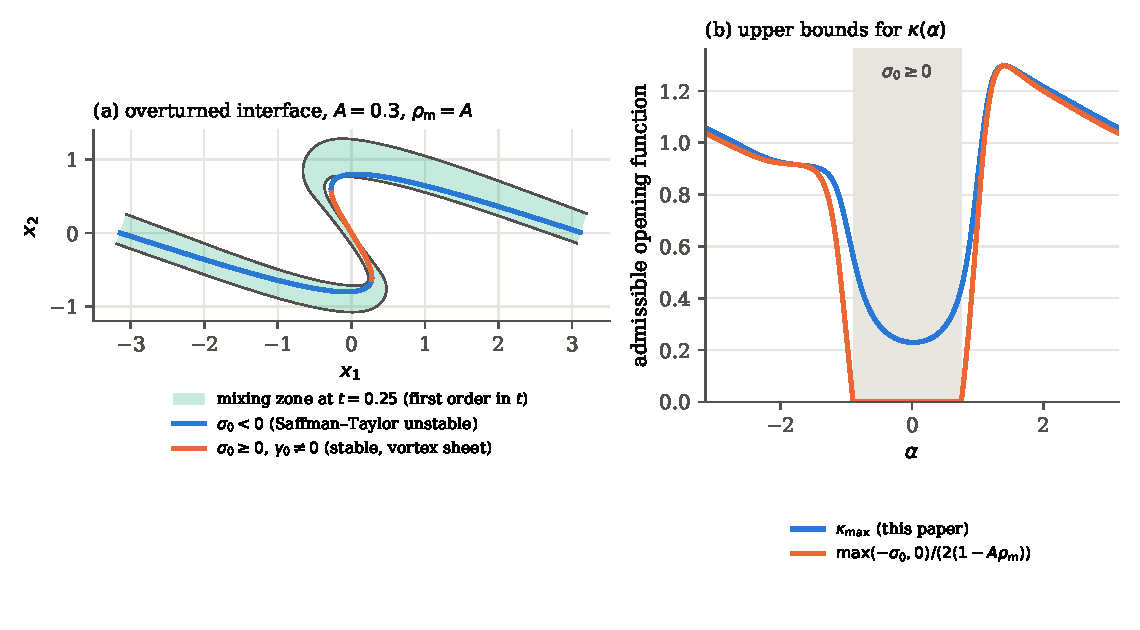
\includegraphics[width=\textwidth]{fig-turned.pdf}
\caption{Overturned interface $z_0(\alpha)=(\alpha-1.5\sin\alpha,0.8\sin\alpha)$ with $A=0.3$ and $\rhom=A$. (a) The initial interface $z_0$, with its Saffman--Taylor stable part $\{\sig_0\ge0\}$
marked in grey, and the strip between $z_0+t(U_0\pm(1\pm\rhom)\kappa)n_0$ for $\kappa=0.8\,\kmax$, i.e.\ the first order part in $t$ of the mixing zone of Theorem~\ref{thm:A}, with its central curve
$z_0+tU_0n_0$. The strip extends along the whole moving interface, including the part where $\sig_0\ge0$; since it is centred on the moving central curve, it does not contain all of $z_0$. The time
$t=0.25$ is illustrative: we have not checked that it is smaller than the existence time $T$ of Theorem~\ref{thm:A}. (b) Single-strip upper bounds for the opening function, as functions of $\alpha$:
$\kmax$ of Theorem~\ref{thm:A}, obtained with the optimal tilt $\delta_*$; the bound $\kappa_{\rm LM}$ of the single layer of \cite{LM26} with its exact hull condition \cite[(4.14)]{LM26}, i.e.\ of the
range \eqref{x:LM-range} (dashed), which differs from $\kmax$ by less than $0.2\%$ for $A=0.3$; and the bound $\max(-\sig_0,0)/(2(1-A^2))$ stated in \cite{LM26} ($\bar c<\frac12$), which is also that of
the untilted strip $\delta=0$ and vanishes on the shaded set $\{\sig_0\ge0\}$.}
\label{fig:turned}
\end{figure}

% ============================================================
\section{Remarks and open problems}\label{sec:remarks}
% ============================================================

\subsection{Consistency with the case $A=0$}
For $A=0$ we have $\sig_0=-2n_{0,2}$ and \eqref{eq:kappa-range} reads $0<\kappa<n_{0,2}$. The strip has normal width $2t\kappa$, i.e.\ vertical width $2t\kappa/n_{0,2}<2t$ (the curves are graphs).
This is consistent with the maximal vertical opening speed $2$ of the mixing zone for equal viscosities in our normalisation \cite{Ott99,Sze12,CCF21,FS18}.

\subsection{Optimal opening rates (formal)}
Single-strip subsolutions do not exhaust the relaxation. Consider instead a mixing zone of width $O(t)$ around $Z$ in which the density has a continuous profile $\bar\rho=R(\xi)$, $\xi=(x-Z)\cdot n/t$,
$R$ increasing from $-1$ at $\xi_-$ to $1$ at $\xi_+$, normalised so that $Z$ is the centre of mass, $\int_{\xi_-}^{\xi_+}\xi R'(\xi)\dd\xi=0$. Repeating the computations of Section~\ref{sec:proof} at leading
order (the conservation law now determines the normal component of $D$ by an integration across the zone instead of the boundary fluxes \eqref{eq:Fplus}--\eqref{eq:Fminus}), one finds, with
$\mathcal P(\xi):=-\int_{\xi_-}^{\xi}\eta R'(\eta)\dd\eta\ge0$ and $D\cdot\tau=0$,
\[
D\cdot n=-\sig-\frac{2(1-AR)\,\mathcal P}{1-R^2},\qquad a\cdot n=-\frac{\sig}{2}-\frac{A^2\mathcal P}{1+AR},
\]
and $D\cdot(D-2a)<0$ if and only if $(1-AR)\mathcal P<-\frac{\sig}2(1-R^2)$ on the zone. The extremal profile $\mathcal P=-\frac\sig2\frac{1-R^2}{1-AR}$ corresponds to $\xi=\frac{\sig}{2}F_1'(R)$ with
$F_1$ as in Example~\ref{ex:flat}, whose fronts are at
\[
\xi_+=-\frac{\sig}{1-A},\qquad \xi_-=\frac{\sig}{1+A}.
\]
Thus, formally, the upper and lower boundaries of the mixing zone may move away from the central interface with normal speeds up to $-\sig/(1-A)$ and $-\sig/(1+A)$, and the width may grow at any
rate below $-2\sig/(1-A^2)$. For the flat interface ($\sig=-2$) this is Example~\ref{ex:flat} with $\theta\to1$. By analogy with \cite[Section~5]{FS18}, we expect that piecewise constant subsolutions with
finitely many intermediate densities approximate these rates, and that the proof of Theorem~\ref{thm:main} extends to them with the same use of $(I-2A\Kop(z_0))^{-1}$.

\subsection{The role of the Saffman--Taylor function}
The proof shows that, at the level of subsolutions, the Saffman--Taylor function plays three roles at once: it is the density of the source part of the Darcy field (so that the field of the
subsolution is linear in $\sig$), it bounds the admissible opening rate, and it is the unknown of the only operator that has to be inverted. The gravitational and viscous contributions to the instability
enter only through $\sig=-2(n_2+AU)$, which is why the mixing zone of Example~\ref{ex:flat} is asymmetric: the relaxed flux is weighted by the mobility $1/(1-A\rho)$, in the spirit of the Koval model for miscible
viscous fingering \cite{Kov63,MO05}.

\subsection{Open problems}
\begin{enumerate}[label=(\arabic*),leftmargin=*]
\item \emph{Partially unstable data.} If $\sig_0$ changes sign, mixing should only occur where $\sig_0<0$, as in \cite{CFM22} for $A=0$. This requires $\kappa$ to vanish at the boundary of the unstable region,
which is excluded by the lower bound $\min\kappa>0$ used in Lemma~\ref{lem:stream}.
\item \emph{Longer times.} The time expansion only gives a short existence time. Continuing the construction requires an evolution equation for the central interface, as in \cite{CCF21,ACF21}; when $A\neq0$
it should involve the averaged version of $(I-2A\Kop)^{-1}$ along the mixing zone.
\item \emph{Regularity.} We assumed $z_0\in C^{6,\gamma}$, which is far from the $C^{3,\alpha}$ of \cite{FS18} for $A=0$. The losses come from the crude bookkeeping in Lemma~\ref{lem:timereg}.
\item \emph{Selection.} For $A=0$, Otto's relaxation selects the maximal mixing rate \cite{Ott99,Sze12}; it would be interesting to know whether a similar selection principle singles out the rates of the previous
subsection when $A\neq0$, see \cite{Men22} for the flat case.
\end{enumerate}

\appendix
% ============================================================
\section{Periodic Cauchy integrals}\label{app:cauchy}
% ============================================================

It is convenient to work with complex densities. For $z\in\Zc^{1,\gamma}$ and $G\in C^{0,\gamma}(\T;\C)$ set
\[
\mathfrak c[z;G](x):=\frac1{4\pi i}\int_\T G(\beta)\,\partial_\beta z(\beta)\cot\frac{z(\beta)-x}{2}\dd\beta,\qquad x\in\C\setminus\Gamma,
\]
so that $\Cf[z;f]^\flat=\mathfrak c[z;f^\flat]$.

\subsection{Reduction to closed curves}
With $w=e^{ix}$ and $\omega=e^{i\zeta}$, a direct computation gives
\[
\tfrac12\cot\tfrac{\zeta-x}{2}\dd\zeta=\frac{\dd\omega}{\omega-w}-\frac i2\dd\zeta .
\]
The map $x\mapsto e^{ix}$ sends the cylinder $\T\times\R$ to $\C\setminus\{0\}$, $\Gamma$ to a closed Jordan curve $\gamma$ of class $C^{k,\gamma}$ winding once around the origin, $\Omega^+(z)$ to the
punctured interior of $\gamma$ and $\Omega^-(z)$ to its exterior. Hence $\mathfrak c[z;G]$ is the classical Cauchy integral $\frac1{2\pi i}\int_\gamma\frac{\tilde G(\omega)\dd\omega}{\omega-w}$ of the
transported density $\tilde G$, minus the constant $\frac1{4\pi}\int_\T G\partial_\beta z\dd\beta$. The classical Plemelj--Privalov theorem for closed $C^{1,\gamma}$ curves
\cite[Chapter~2]{Mus53}, \cite[Chapter~7]{Kre14} then gives Lemma~\ref{lem:cauchy}(b): $\mathfrak c[z;G]$ extends to a $C^{0,\gamma}$ function on each closed region, with norm bounded by
$C\|G\|_{C^{0,\gamma}}$, where $C$ depends only on $\gamma$, $\delta(z)$ and $\|z\|_{\Zc^{1,\gamma}}$; its boundary values are given by the Plemelj formulas
$\mathfrak c^\pm=\pm\frac12G+\pv\,\mathfrak c$. The value at $w=0$ corresponds to the limit $x_2\to+\infty$.

\subsection{Derivative identities}
\begin{lemma}\label{lem:identities}
Let $z\in\Zc^{2,\gamma}$ and $G\in C^{1,\gamma}(\T;\C)$. Then, in $\C\setminus\Gamma$,
\begin{equation}\label{eq:dx}
\partial_x\,\mathfrak c[z;G]=\mathfrak c\Big[z;\frac{\partial_\beta G}{\partial_\beta z}\Big].
\end{equation}
If $z=z(\beta,t)$ and $G=G(\beta,t)$ are $C^1$ in $t$ with values in $\Zc^{2,\gamma}$ and $C^{1,\gamma}$, then
\begin{equation}\label{eq:dt}
\partial_t\,\mathfrak c[z;G](x)=\mathfrak c\Big[z;\partial_tG-\frac{\partial_\beta G}{\partial_\beta z}\,\partial_tz\Big](x),\qquad x\notin\Gamma(t).
\end{equation}
\end{lemma}

\begin{proof}
Since $\partial_\beta\cot\frac{z(\beta)-x}2=-\frac12\csc^2\frac{z(\beta)-x}2\,\partial_\beta z$, we have $\partial_x\cot\frac{z(\beta)-x}2=-\partial_\beta\cot\frac{z(\beta)-x}2/\partial_\beta z$ and
$\partial_t\cot\frac{z(\beta)-x}2=\partial_\beta\cot\frac{z(\beta)-x}2\cdot\partial_tz/\partial_\beta z$. Integrating by parts in $\beta$ (there are no boundary terms by periodicity),
\[
\partial_x\mathfrak c=-\frac1{4\pi i}\int G\,\partial_\beta\cot\dd\beta=\frac1{4\pi i}\int\partial_\beta G\cot\dd\beta,
\]
which is \eqref{eq:dx}, and
\[
\partial_t\mathfrak c=\frac1{4\pi i}\int\Big[(\partial_tG\,\partial_\beta z+G\,\partial_\beta\partial_tz)\cot-\partial_\beta(G\partial_tz)\cot\Big]\dd\beta
=\frac1{4\pi i}\int\big(\partial_tG\,\partial_\beta z-\partial_\beta G\,\partial_tz\big)\cot\dd\beta,
\]
which is \eqref{eq:dt}.
\end{proof}

Iterating \eqref{eq:dx} and using the Plemelj--Privalov theorem gives Lemma~\ref{lem:cauchy}(d): if $z\in\Zc^{j+1,\gamma}$ and $G\in C^{j,\gamma}$ then all derivatives of order $\le j$ of $\mathfrak c[z;G]$ are
Cauchy integrals of $C^{0,\gamma}$ densities, hence $C^{0,\gamma}$ up to $\Gamma$. If $x=x(t)$ is a $C^1$ path in $\Omega^\pm(z(t))$, then since $\mathfrak c$ is holomorphic,
\begin{equation}\label{eq:chain}
\frac{\dd}{\dd t}\,\mathfrak c[z;G]\big(x(t)\big)=\mathfrak c\Big[z;\partial_tG-\frac{\partial_\beta G}{\partial_\beta z}\partial_tz\Big](x)+\mathfrak c\Big[z;\frac{\partial_\beta G}{\partial_\beta z}\Big](x)\;\dot x,
\end{equation}
and by uniform convergence of the derivatives up to $\Gamma$ the same formula holds for the boundary values $t\mapsto\mathfrak c[z;G]^\pm(\alpha)$ with $x(t)=z(\alpha,t)$.

\subsection{Continuity}
\begin{lemma}\label{lem:continuity}
Let $z_k\to z$ in $\Zc^{1,\gamma}$ and $G_k\to G$ in $C^{0,\gamma}(\T;\C)$. Then $\mathfrak c[z_k;G_k]^\pm\to\mathfrak c[z;G]^\pm$ uniformly on $\T$, and if $x_k\in\overline{\Omega^+(z_k)}$ with $x_k\to z(\alpha)$, then
$\mathfrak c[z_k;G_k](x_k)\to\mathfrak c[z;G]^+(\alpha)$; similarly from below.
\end{lemma}

\begin{proof}
By the Plemelj--Privalov theorem the functions $\mathfrak c_k:=\mathfrak c[z_k;G_k]$ are uniformly $C^{0,\gamma}$ on $\overline{\Omega^+(z_k)}$, with a constant $L$ independent of $k$. Given $\eps>0$ let
$y=z(\alpha)+\eps n(\alpha)$; for $k$ large $y\in\Omega^+(z_k)$ at distance $\ge\eps/2$ from $\Gamma_k$, so $\mathfrak c_k(y)\to\mathfrak c[z;G](y)$ by dominated convergence. Hence
\[
\limsup_k|\mathfrak c_k(x_k)-\mathfrak c[z;G]^+(\alpha)|\le\limsup_k\big(L|x_k-y|^\gamma+L\eps^\gamma\big)\le 2L\eps^\gamma,
\]
and $\eps$ is arbitrary. Uniformity in $\alpha$ follows from the same argument and the equicontinuity.
\end{proof}

\subsection{Proof of Lemma~\ref{lem:timereg} and of the regularity of $G$ in Lemma~\ref{lem:accel}}
By Lemma~\ref{lem:geometry}, the curves $z^\pm(\cdot,t)$ are polynomials in $t$ with coefficients in $C^{3,\gamma}$, with $\delta(z^\pm)\ge\frac12\delta(z_0)$ on $[0,T_1]$. The normals $n^\pm$, the lengths
$|\partial_\alpha z^\pm|$ and the velocities $V^\pm=\partial_tz^\pm\cdot n^\pm$ are therefore smooth in $t$ with values in $C^{2,\gamma}$, and so are the complex densities $G^\pm:=(f^\pm)^\flat$ and their time
derivatives.

By \eqref{eq:vS}, $(v_S^+)^\flat=\mathfrak c[z^+;G^+]^-+\mathfrak c[z^-;G^-]\circ z^+$, where $z^+(\alpha,t)\in\Omega^+(z^-(\cdot,t))$ for $t>0$, and similarly for $v_S^-$. Applying \eqref{eq:chain} once, $\partial_tv_S^\pm$
is a sum of boundary values and evaluations on the other curve of Cauchy integrals with densities
\[
G_1^\pm=\partial_tG^\pm-\frac{\partial_\beta G^\pm}{\partial_\beta z^\pm}\partial_tz^\pm,\qquad G_2^\pm=\frac{\partial_\beta G^\pm}{\partial_\beta z^\pm},
\]
multiplied by $\partial_tz^\pm$; these densities are bounded in $C^{1,\gamma}$ uniformly in $t$. Applying \eqref{eq:chain} once more, $\partial_t^2v_S^\pm$ involves Cauchy integrals of densities bounded in
$C^{0,\gamma}$, evaluated on $\Gamma^\pm(t)$ from the side of the strip, and these are bounded uniformly in $t\in(0,T_1]$ by the Plemelj--Privalov theorem. Since $F^\pm$ are polynomials in
$v_S^\pm\cdot n^\pm$, $V^\pm$, $n_2^\pm$ and $|\partial_\alpha z^\pm|$, we obtain that $\partial_tF^\pm$ and $\partial_t^2F^\pm$ are bounded in $C^0(\T)$ on $(0,T_1]$. By Lemma~\ref{lem:continuity} applied to the
densities appearing in $F^\pm$ and $\partial_tF^\pm$, these functions extend continuously to $t=0$, which proves the first part of Lemma~\ref{lem:timereg}.

For \eqref{eq:v-strip}, let $x=X(\alpha,\lambda,t)$, so that $|x-z^\pm(\alpha,t)|\le2t\kappa(\alpha)$. The uniform Hölder bounds on $\overline{\Omega^-(z^+)}$ and $\overline{\Omega^+(z^-)}$ give
$|v(x,t)-v_S^+(\alpha,t)|\le Ct^\gamma$, and the Lipschitz bound in time just proved gives $|v_S^+(\alpha,t)-v_S^{(0)}(\alpha)|\le Ct$.

Finally, $G=\partial_tM(\cdot,0)$ for $a=0$, $h=0$ is obtained by letting $t\to0$ in the formula for $\partial_tM$. In the limit all Cauchy integrals become boundary values on $z_0\in\Zc^{6,\gamma}$, and
the densities involve $n_0\in C^{5,\gamma}$, $\partial_tz^\pm(\cdot,0)=(U_0\pm c^\pm)n_0\in C^{4,\gamma}$, their first $\alpha$-derivatives, and $\partial_t^2z^\pm(\cdot,0)=0$. Thus
$G^\pm(\cdot,0)\in C^{4,\gamma}$, $G_1^\pm(\cdot,0),G_2^\pm(\cdot,0)\in C^{3,\gamma}$, and by Lemma~\ref{lem:cauchy}(d) the boundary values are in $C^{3,\gamma}$. The remaining factors ($\partial_tz^\pm(\cdot,0)$, $n_0$,
and the time derivatives at $t=0$ of $n^\pm$, $V^\pm$ and $|\partial_\alpha z^\pm|$, which involve $\partial_\alpha\partial_tz^\pm(\cdot,0)$) belong to $C^{3,\gamma}$. Hence $G\in C^{3,\gamma}(\T)$.
\qed


\begin{thebibliography}{99}

\bibitem[Amb04]{Amb04}
D.~M. Ambrose, \emph{Well-posedness of two-phase Hele-Shaw flow without surface tension}, European J. Appl. Math. \textbf{15} (2004), no.~5, 597--607.

\bibitem[ACF21]{ACF21}
V.~Arnaiz, \'A.~Castro, D.~Faraco, \emph{Semiclassical estimates for pseudodifferential operators and the Muskat problem in the unstable regime},
Comm. Partial Differential Equations \textbf{46} (2021), no.~1, 135--164.

\bibitem[CCF21]{CCF21}
\'A.~Castro, D.~C\'ordoba, D.~Faraco, \emph{Mixing solutions for the Muskat problem}, Invent. Math. \textbf{226} (2021), 251--348.

\bibitem[CFM19]{CFM19}
\'A.~Castro, D.~Faraco, F.~Mengual, \emph{Degraded mixing solutions for the Muskat problem}, Calc. Var. Partial Differential Equations \textbf{58} (2019), Paper No.~58.

\bibitem[CFM22]{CFM22}
\'A.~Castro, D.~Faraco, F.~Mengual, \emph{Localized mixing zone for Muskat bubbles and turned interfaces}, Ann. PDE \textbf{8} (2022).

\bibitem[CCG11]{CCG11}
A.~C\'ordoba, D.~C\'ordoba, F.~Gancedo, \emph{Interface evolution: the Hele-Shaw and Muskat problems}, Ann. of Math. (2) \textbf{173} (2011), no.~1, 477--542.

\bibitem[CFG11]{CFG11}
D.~C\'ordoba, D.~Faraco, F.~Gancedo, \emph{Lack of uniqueness for weak solutions of the incompressible porous media equation}, Arch. Ration. Mech. Anal. \textbf{200} (2011), no.~3, 725--746.

\bibitem[CG07]{CG07}
D.~C\'ordoba, F.~Gancedo, \emph{Contour dynamics of incompressible 3-D fluids in a porous medium with different densities}, Comm. Math. Phys. \textbf{273} (2007), no.~2, 445--471.

\bibitem[DLS09]{DLS09}
C.~De~Lellis, L.~Sz\'ekelyhidi~Jr., \emph{The Euler equations as a differential inclusion}, Ann. of Math. (2) \textbf{170} (2009), no.~3, 1417--1436.

\bibitem[FS18]{FS18}
C.~F\"orster, L.~Sz\'ekelyhidi~Jr., \emph{Piecewise constant subsolutions for the Muskat problem}, Comm. Math. Phys. \textbf{363} (2018), no.~3, 1051--1080.

\bibitem[Gan17]{Gan17}
F.~Gancedo, \emph{A survey for the Muskat problem and a new estimate}, SeMA J. \textbf{74} (2017), no.~1, 21--35.

\bibitem[GBL20]{GBL20}
R.~Granero-Belinch\'on, O.~Lazar, \emph{Growth in the Muskat problem}, Math. Model. Nat. Phenom. \textbf{15} (2020).

\bibitem[GKS21]{GKS21}
B.~Gebhard, J.~J. Kolumb\'an, L.~Sz\'ekelyhidi~Jr., \emph{A new approach to the Rayleigh--Taylor instability}, Arch. Ration. Mech. Anal. \textbf{241} (2021), no.~3, 1243--1280.

\bibitem[Hom87]{Hom87}
G.~M. Homsy, \emph{Viscous fingering in porous media}, Annu. Rev. Fluid Mech. \textbf{19} (1987), 271--311.

\bibitem[KMS03]{KMS03}
B.~Kirchheim, S.~M\"uller, V.~\v{S}ver\'ak, \emph{Studying nonlinear PDE by geometry in matrix space}, in: Geometric Analysis and Nonlinear Partial Differential Equations, Springer, Berlin, 2003, 347--395.

\bibitem[Kov63]{Kov63}
E.~J. Koval, \emph{A method for predicting the performance of unstable miscible displacement in heterogeneous media}, Soc. Petrol. Eng. J. \textbf{3} (1963), no.~2, 145--154.

\bibitem[Kre14]{Kre14}
R.~Kress, \emph{Linear Integral Equations}, 3rd ed., Applied Mathematical Sciences \textbf{82}, Springer, New York, 2014.

\bibitem[LM26]{LM26}
P.~Luna, F.~Mengual, \emph{Mixing solutions for unstable Muskat data with viscosity jump}, talk (abstract) at the Seminario EDPs y Mec\'anica de Fluidos, ICMAT, Madrid, 12 November 2026.

\bibitem[Mat19]{Mat19}
B.-V. Matioc, \emph{The Muskat problem in two dimensions: equivalence of formulations, well-posedness, and regularity results}, Anal. PDE \textbf{12} (2019), no.~2, 281--332.

\bibitem[Men22]{Men22}
F.~Mengual, \emph{H-principle for the 2-dimensional incompressible porous media equation with viscosity jump}, Anal. PDE \textbf{15} (2022), no.~2, 429--476.

\bibitem[MO05]{MO05}
G.~Menon, F.~Otto, \emph{Dynamic scaling in miscible viscous fingering}, Comm. Math. Phys. \textbf{257} (2005), no.~2, 303--317.

\bibitem[MS23]{MS23}
F.~Mengual, L.~Sz\'ekelyhidi~Jr., \emph{Dissipative Euler flows for vortex sheet initial data without distinguished sign}, Comm. Pure Appl. Math. \textbf{76} (2023), no.~1, 163--221.

\bibitem[Mus34]{Mus34}
M.~Muskat, \emph{Two fluid systems in porous media. The encroachment of water into an oil sand}, Physics \textbf{5} (1934), 250--264.

\bibitem[Mus53]{Mus53}
N.~I. Muskhelishvili, \emph{Singular Integral Equations}, P. Noordhoff, Groningen, 1953.

\bibitem[NP20]{NP20}
H.~Q. Nguyen, B.~Pausader, \emph{A paradifferential approach for well-posedness of the Muskat problem}, Arch. Ration. Mech. Anal. \textbf{237} (2020), no.~1, 35--100.

\bibitem[NS21]{NS21}
F.~Noisette, L.~Sz\'ekelyhidi~Jr., \emph{Mixing solutions for the Muskat problem with variable speed}, J. Evol. Equ. \textbf{21} (2021).

\bibitem[Ott99]{Ott99}
F.~Otto, \emph{Evolution of microstructure in unstable porous media flow: a relaxational approach}, Comm. Pure Appl. Math. \textbf{52} (1999), no.~7, 873--915.

\bibitem[SCH04]{SCH04}
M.~Siegel, R.~E. Caflisch, S.~Howison, \emph{Global existence, singular solutions, and ill-posedness for the Muskat problem}, Comm. Pure Appl. Math. \textbf{57} (2004), no.~10, 1374--1411.

\bibitem[Shv11]{Shv11}
R.~Shvydkoy, \emph{Convex integration for a class of active scalar equations}, J. Amer. Math. Soc. \textbf{24} (2011), no.~4, 1159--1174.

\bibitem[ST58]{ST58}
P.~G. Saffman, G.~Taylor, \emph{The penetration of a fluid into a porous medium or Hele-Shaw cell containing a more viscous liquid}, Proc. Roy. Soc. London Ser.~A \textbf{245} (1958), 312--329.

\bibitem[Sze12]{Sze12}
L.~Sz\'ekelyhidi~Jr., \emph{Relaxation of the incompressible porous media equation}, Ann. Sci. \'Ec. Norm. Sup\'er. (4) \textbf{45} (2012), no.~3, 491--509.

\end{thebibliography}


\end{document}
